In the previous section we analyzed the presence of sequential dynamical invariants in a CPG model, showing that strong correlations can be formed when stimulating certain neurons in the circuit and only when the circuit modeled has enough flexibility to adapt to the changes in the rhythm. In this section we will explore these phenomena in intracellular recordings of the living activity of the feeding CPG of \textit{Lymnaea stagnalis}. The aim here is to search for sequential dynamical invariants as those reported in \textcite{elices_robust_2019}, and also explore their functional meaning by analyzing different sources of stimulation of the rhythm. The data here characterized was kindly provided for this work by Dr. Michael Crossley, University of Sussex (see Sec. \ref{subsec:methods experimental intervals}).

When studying temporal structures in neural dynamics, the definition of time references is a key first point. In the computational analysis described in the previous section, the time references to define cycle-by-cycle sequence intervals were the first and last spikes of each burst. In that case, as in the case of the pyloric neurons in \textit{C. maenas}, the CPG phases are directly related to the bursting activity of these motoneurons and the burst can be consistently identified by the first and last spike. However, in the case of the feeding CPG in \textit{Lymnaea stagnalis}, the activity is usually characterized with recordings from both interneurons and motoneurons \parencite{elliott_interactions_1985, staras_patterngenerating_1998, benjamin_distributed_2012}. This requires a more complex combination of burst references to characterize the phases of the CPG --protraction, rasp and swallow-- based on cycle-by-cycle time intervals. Thus, for this analysis, we will consider again the three phases of the CPG which are associated mainly to the three interneurons --N1M, N2v and N3t. Since it is not always possible to record these neurons at the same time (specially N2v that is located in the ventral side), we will establish the time references for the sequence analysis by a combination of interneuron and motoneuron events following their activity at each phase. 

\begin{figure}[bth!]
	\centering
	\begin{minipage}[b]{0.7\textwidth}
		\makebox[0pt][l]{\hspace*{-130pt}\text{a)}}\\
		\centering
		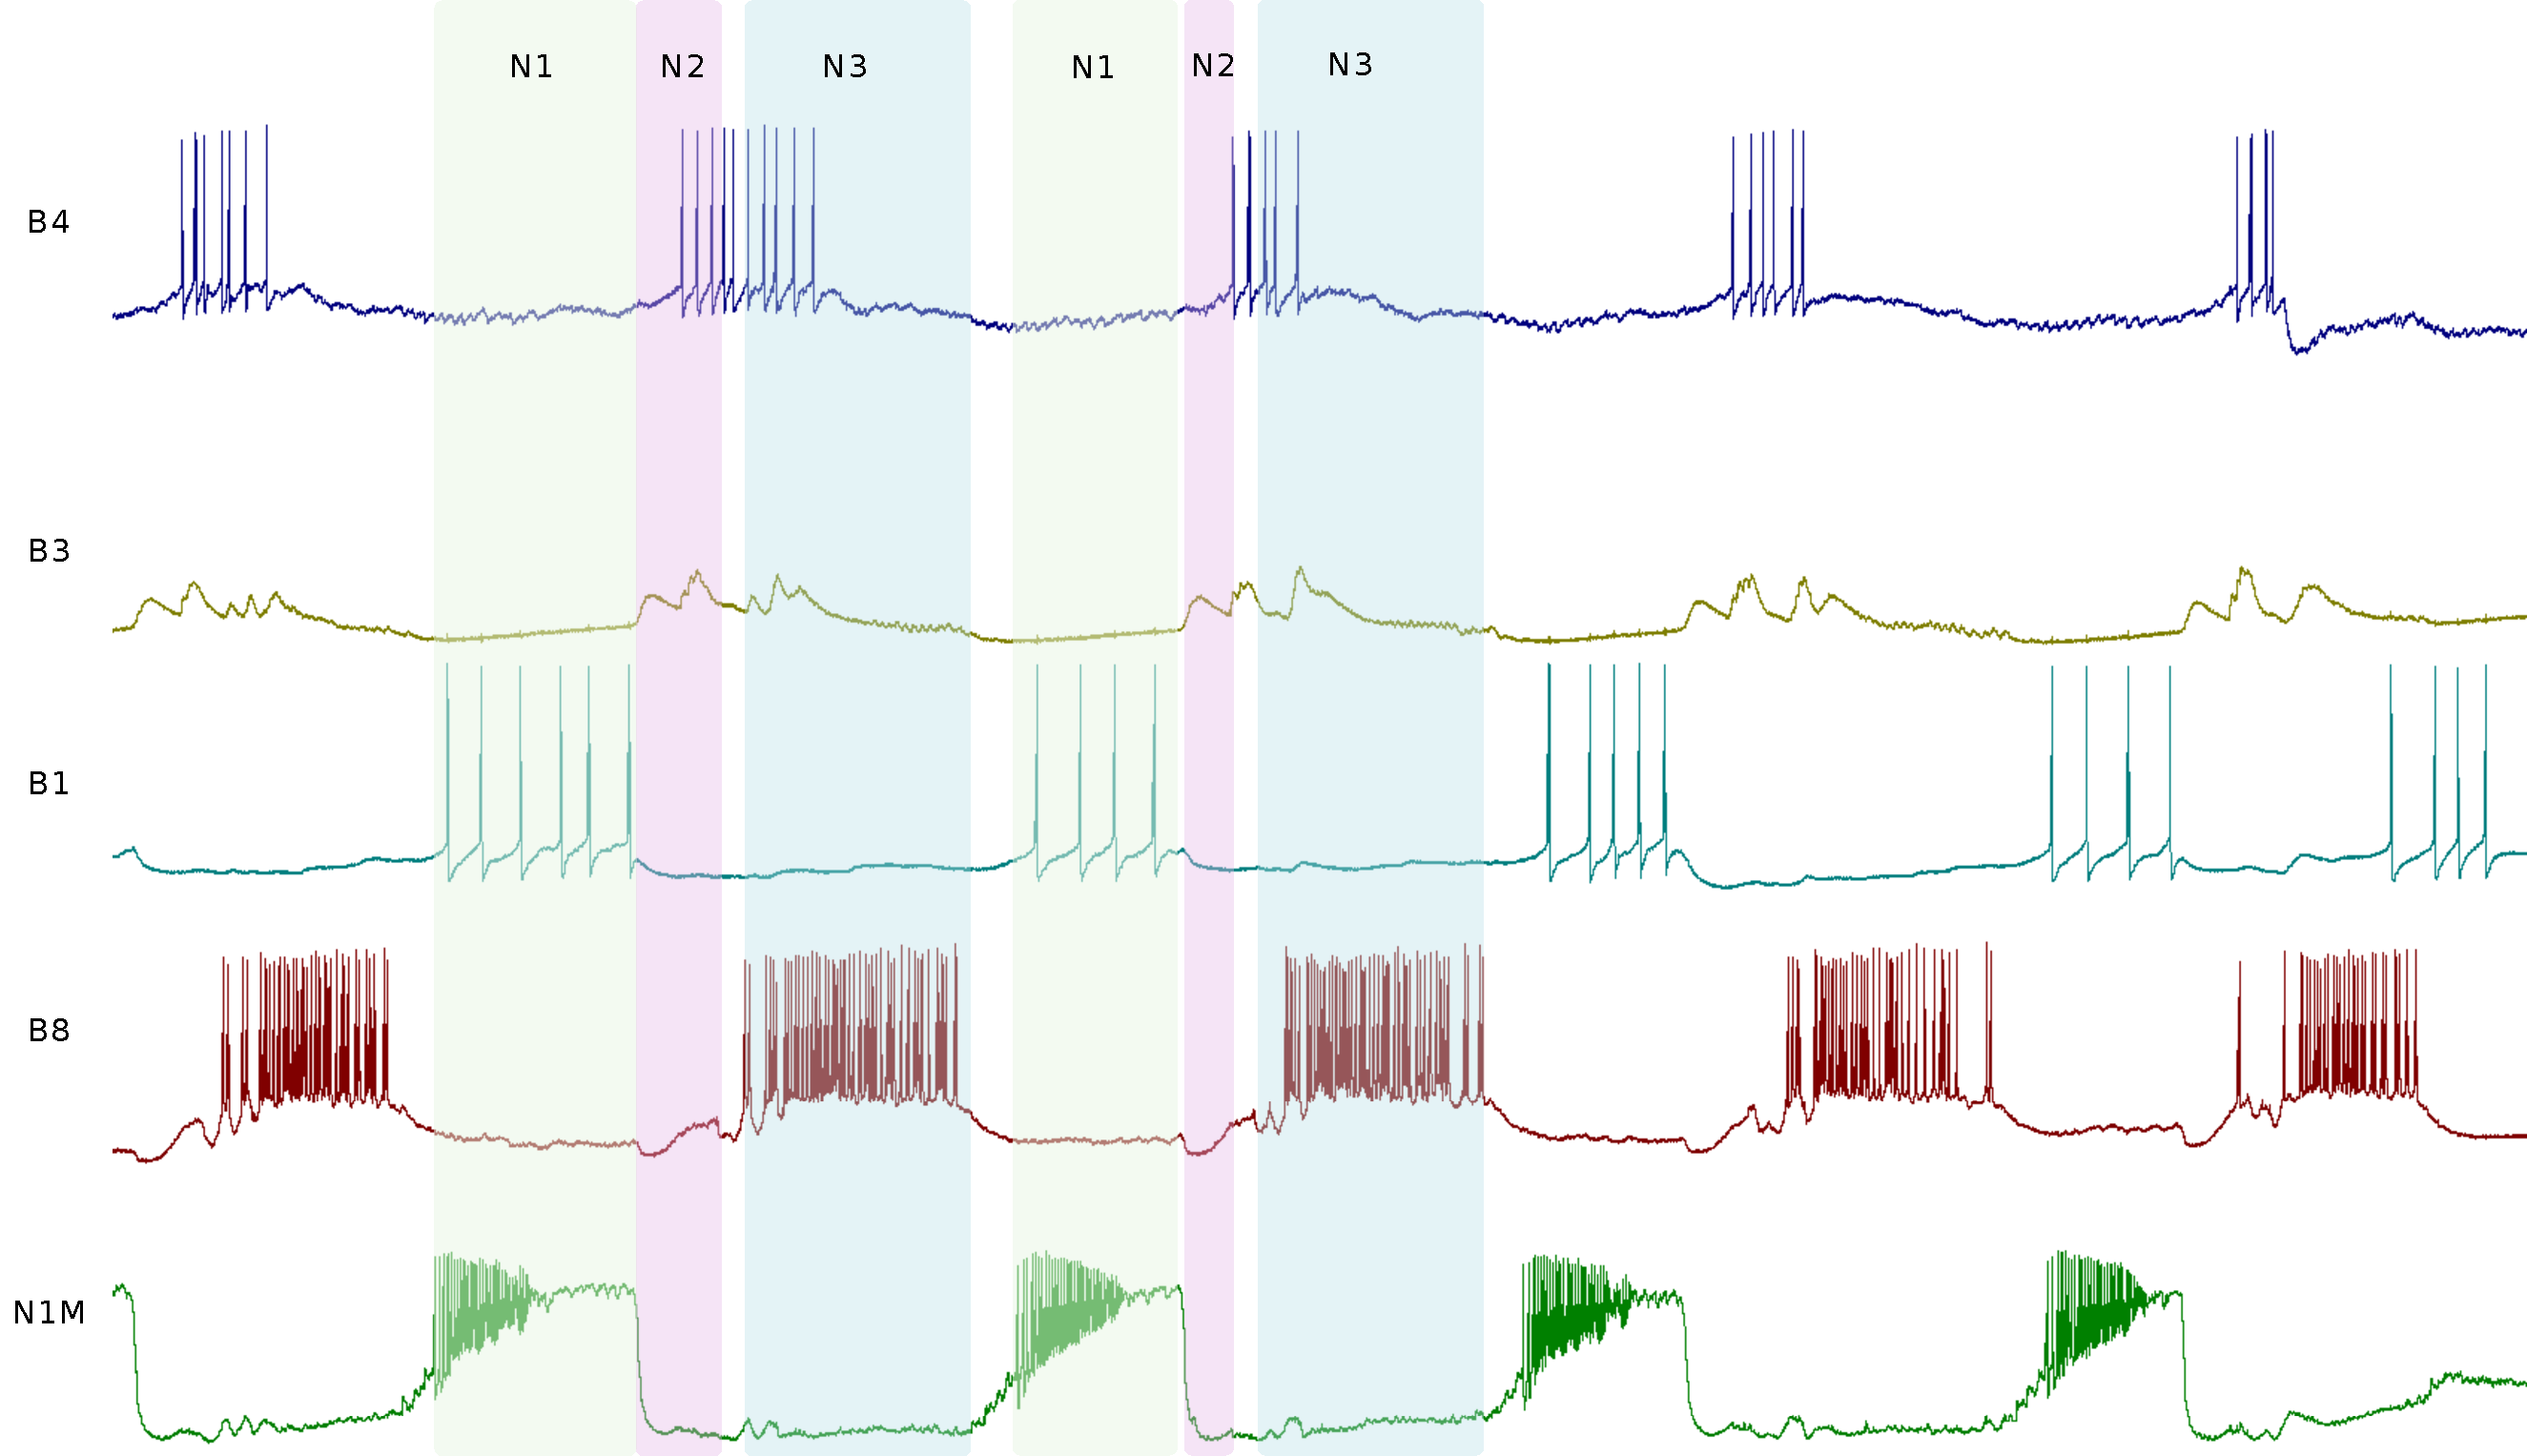
\includegraphics[width=\textwidth]{img/invariants/example_phases_1.pdf}
	\end{minipage}
	\vspace{20pt}
	\begin{minipage}[b]{0.7\textwidth}
		\makebox[0pt][l]{\hspace*{-130pt}\text{b)}}\\
		\centering
		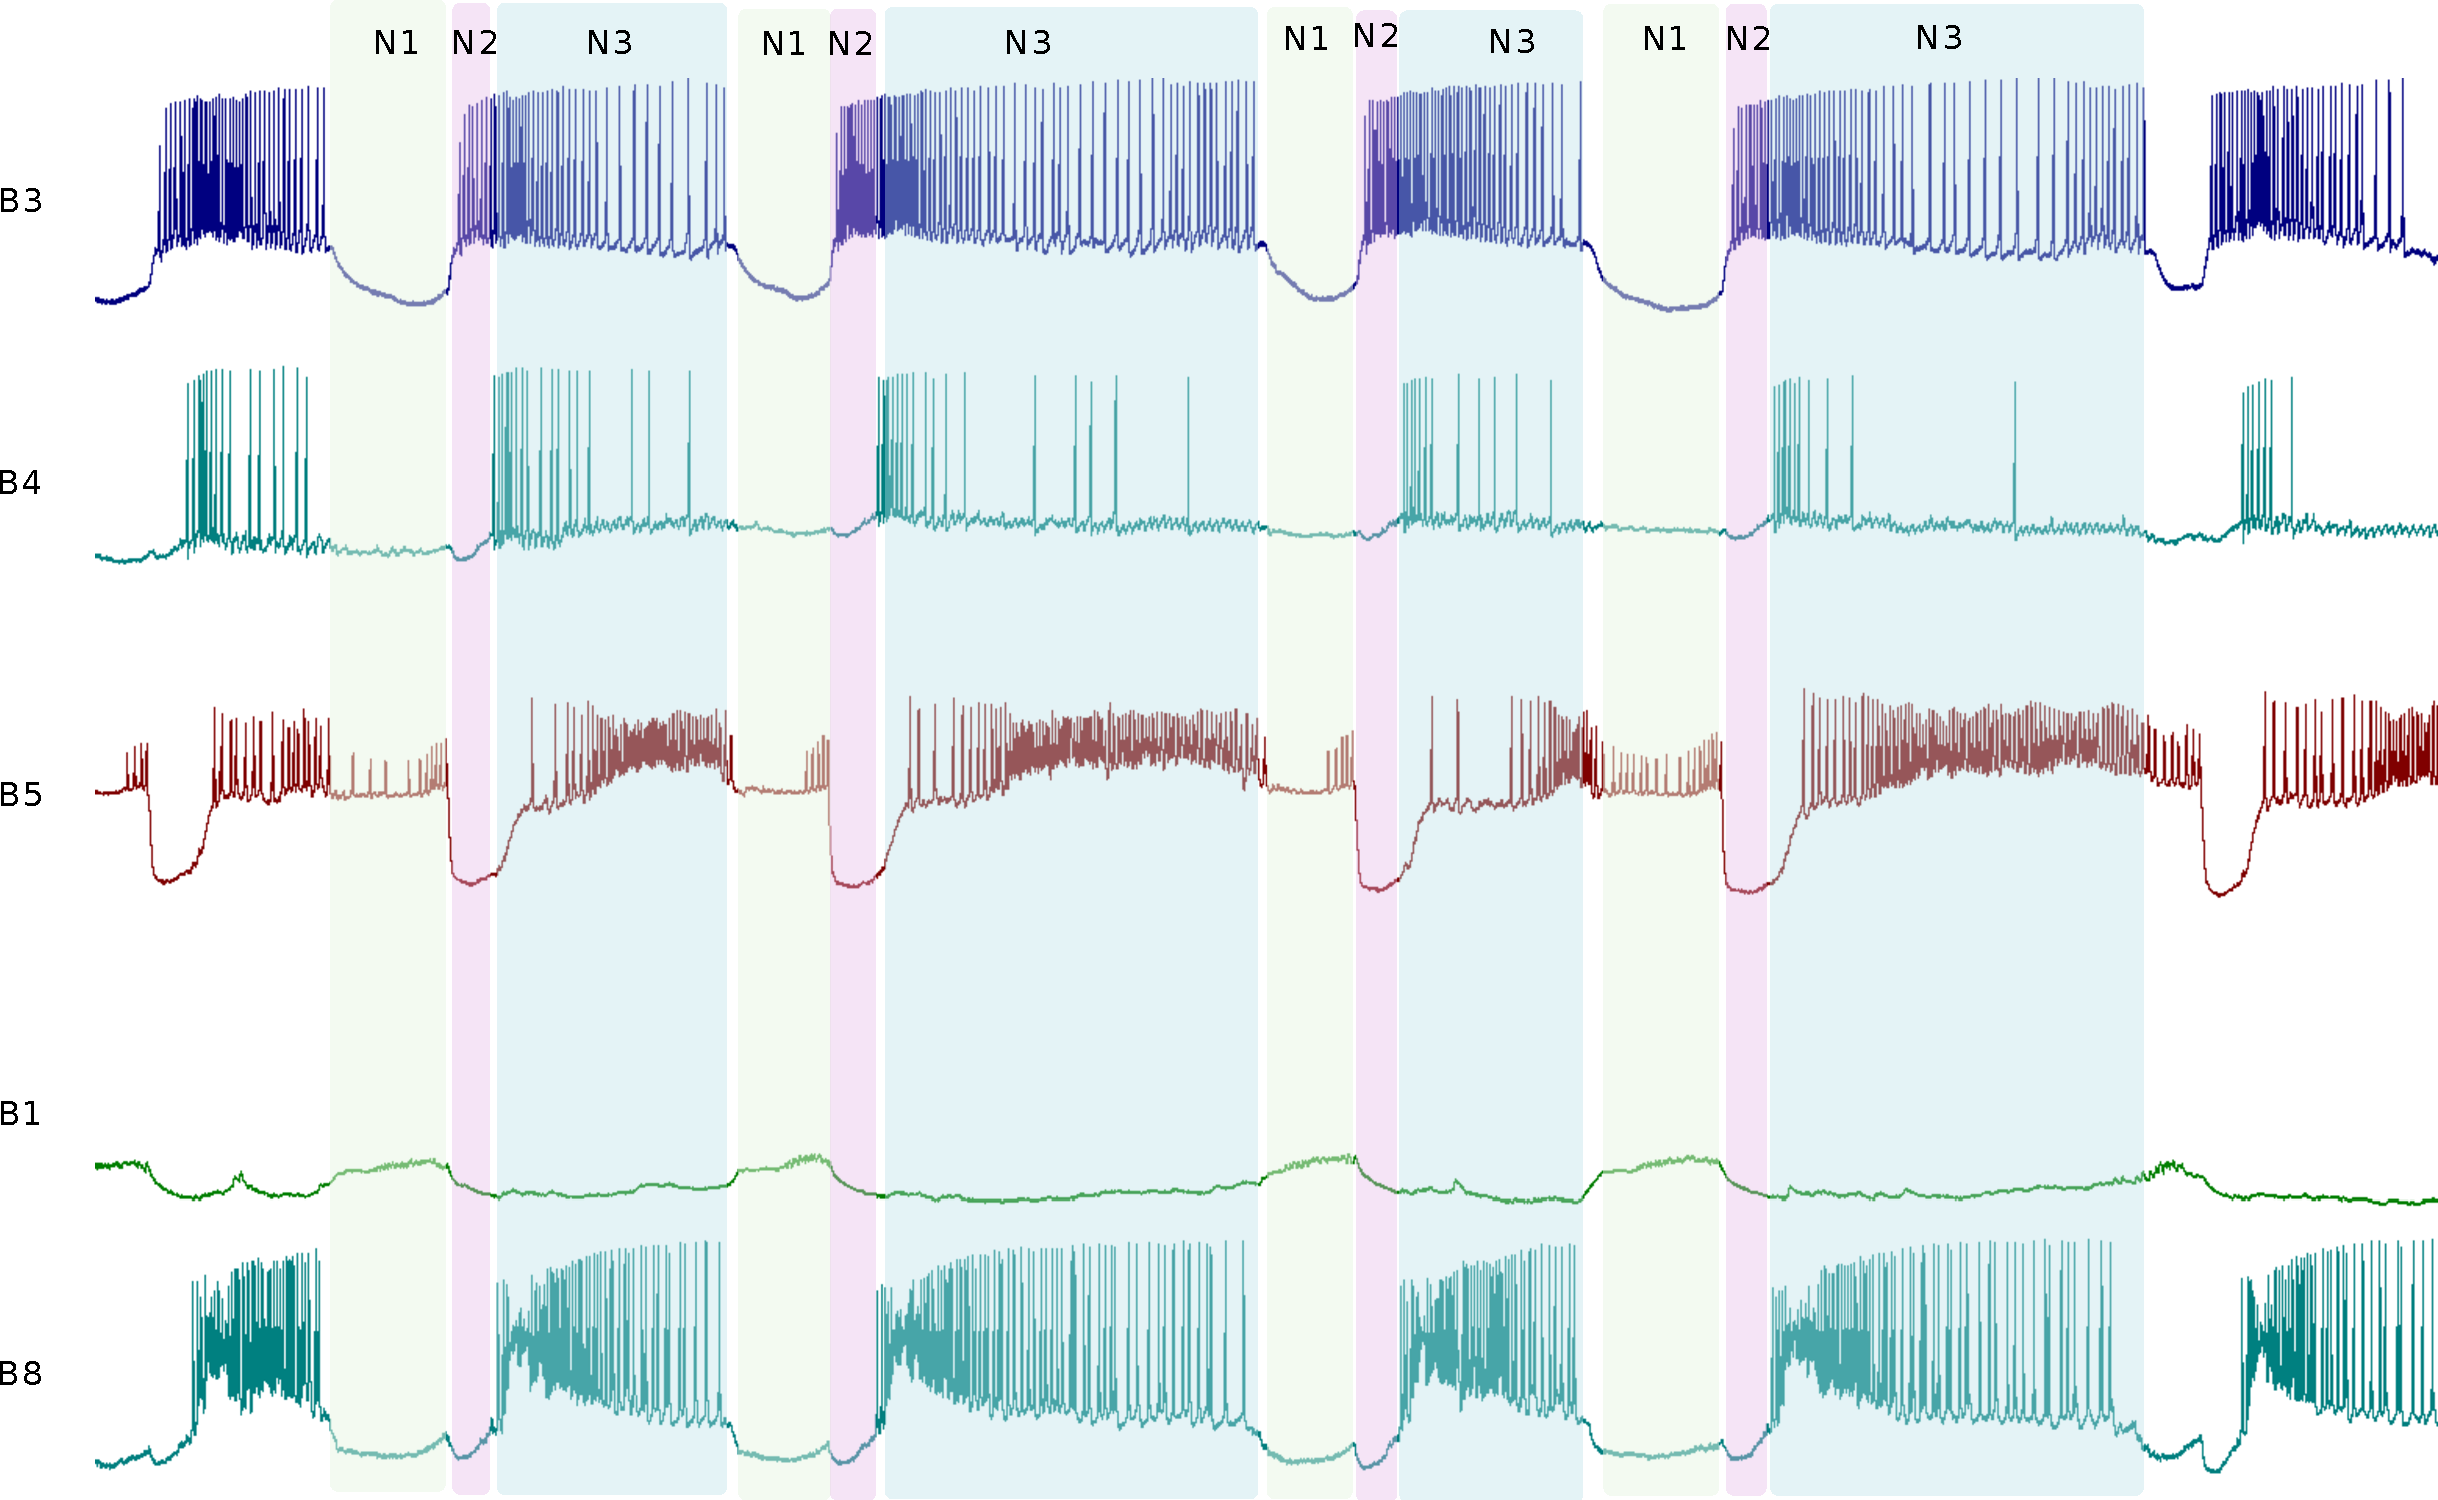
\includegraphics[width=\textwidth]{img/invariants/example_phases_2.pdf}
	\end{minipage}
	\caption{Delimitation of phases in the feeding CPG of \textit{Lymnaea stagnalis} based on different recordings. Panel a) intracellular recordings for motoneurons B4, B3, B1 and B8 and the interneuron N1M. Phases are delimited by N1M and B1, which have the same activation time for phase N1, the inhibition of N1M and the start of the depolarization in B8 for phase N2, and the first and last spike of burst B8 for phase N3. Panel b) intracellular recordings for motoneurons B3, B4, B5, B1 and B8. Phases are delimited by B1 depolarization for phase N1, the strong inhibition of B5 for phase N2, and the first and last spike of burst B8 for phase N3.}
	\label{fig:example lymnaea phases recording}
\end{figure}

For example, in Figure \ref{fig:example lymnaea phases recording} the three phases in the CPG are marked by a colored background over the recording. Note that they can be delimited by the neurons in the circuit but some of the motoneurons cover several phases, as it is the case of B4 in panel a) or B3 in panel b). Phases can also be defined by the first and last spike, as it is the case for phase N3 and neuron B8, but in other cases as the phase N2, the relevant reference is the hyperpolarization of specific neurons, such as the strong inhibition visible in neuron B5 in panel b). Also, the depolarization of some neurons carries relevant information, since, for example in the case of B1 in Fig. \ref{fig:example lymnaea phases recording}.b), the visible depolarizations that did not generate action potentials represent the N1 phase through the connection between N1M and B1. Therefore, to characterize the time sequences in the feeding CPG, we needed compound references from several neural recordings, which are summarized in Table \ref{table:cpg ref intervals}. Note that, different time references must be taken into account to reach conclusions about the time-interval constraints in the cycle-by-cycle analysis. All possible intervals conforming each cycle between the neurons are taken into account in this analysis (see \ref{subsec:intervals}). The events and neural recordings to define each time-interval for each are described in section \ref{subsec:methods experimental intervals} for each experiment.


\begin{table}[htb!]
	\centering
	\begin{tabular}{cl|l|l}
			\multicolumn{1}{l}{}                                 & \multicolumn{1}{c|}{\textbf{N1-Protraction}} & \multicolumn{1}{c|}{\textbf{N2-Rasp}} & \multicolumn{1}{c}{\textbf{N3-Swallow}} \\ \hline
			\multicolumn{1}{c|}{\multirow{3}{*}{\textbf{Start}}} & Last spike of N3t/B3                         & Inhibition of B5                      & First spike of B8                       \\
			\multicolumn{1}{c|}{}                                & Depolarization or first spike in B1          &                                       &                                         \\
			\multicolumn{1}{c|}{}                                & First spike in B6                            &                                       &                                         \\ \hline
			\multicolumn{1}{c|}{\multirow{2}{*}{\textbf{End}}}   & Last spike of B5                             & First spike of B8                     & Last spike of N3t/B3                    \\
			\multicolumn{1}{c|}{}                                & Hyperpolarization in B1 or B6                &                                       &                                        
		\end{tabular}
	\caption{Time reference boundaries for the three phases in the feeding CPG.}
	\label{table:cpg ref intervals}
\end{table}

Another key point in the study of the feeding CPG of \textit{L. stagnalis} is that the generation of the rhythm is a combined action of different cells \parencite{benjamin_distributed_2012}, not only interneurons but also motoneurons have a role in the activation \parencite{staras_patterngenerating_1998}, and modulatory neurons in the buccal and cerebral ganglia are involved in the rhythm. Figure \ref{fig:feeding distribution} shows a diagram with the distributed circuit connections in the CPG and modulatory neurons connected to it. All these factors affect the rhythm and thus the neuronal sequential activation and how variability is distributed among the different intervals cycle by cycle. Also, not all the neurons are involved every time the rhythm is active, and that gives also information about the different contexts in which the rhythm evolves. For example, the rhythm can be activated by the presence of food or sucrose stimulation, in which case the animal needs to initiate the activity and ingest food. Then, the rhythm is started by the stimulation of the lip nerve that also excites N1M neuron. Also, even at the absence of food, when the animal is hungry, the CPG can be activated, in this case with a strong role of N3t as modulator. The modulation of the rhythm is also a key aspect, and modulatory neurons such as SO or CV1a control the rhythm after its initiation, and they have shown to have distinct alternative roles in the activity \parencite{kemenes_multiple_2001}. 

\begin{figure}[bth!]
	\centering
	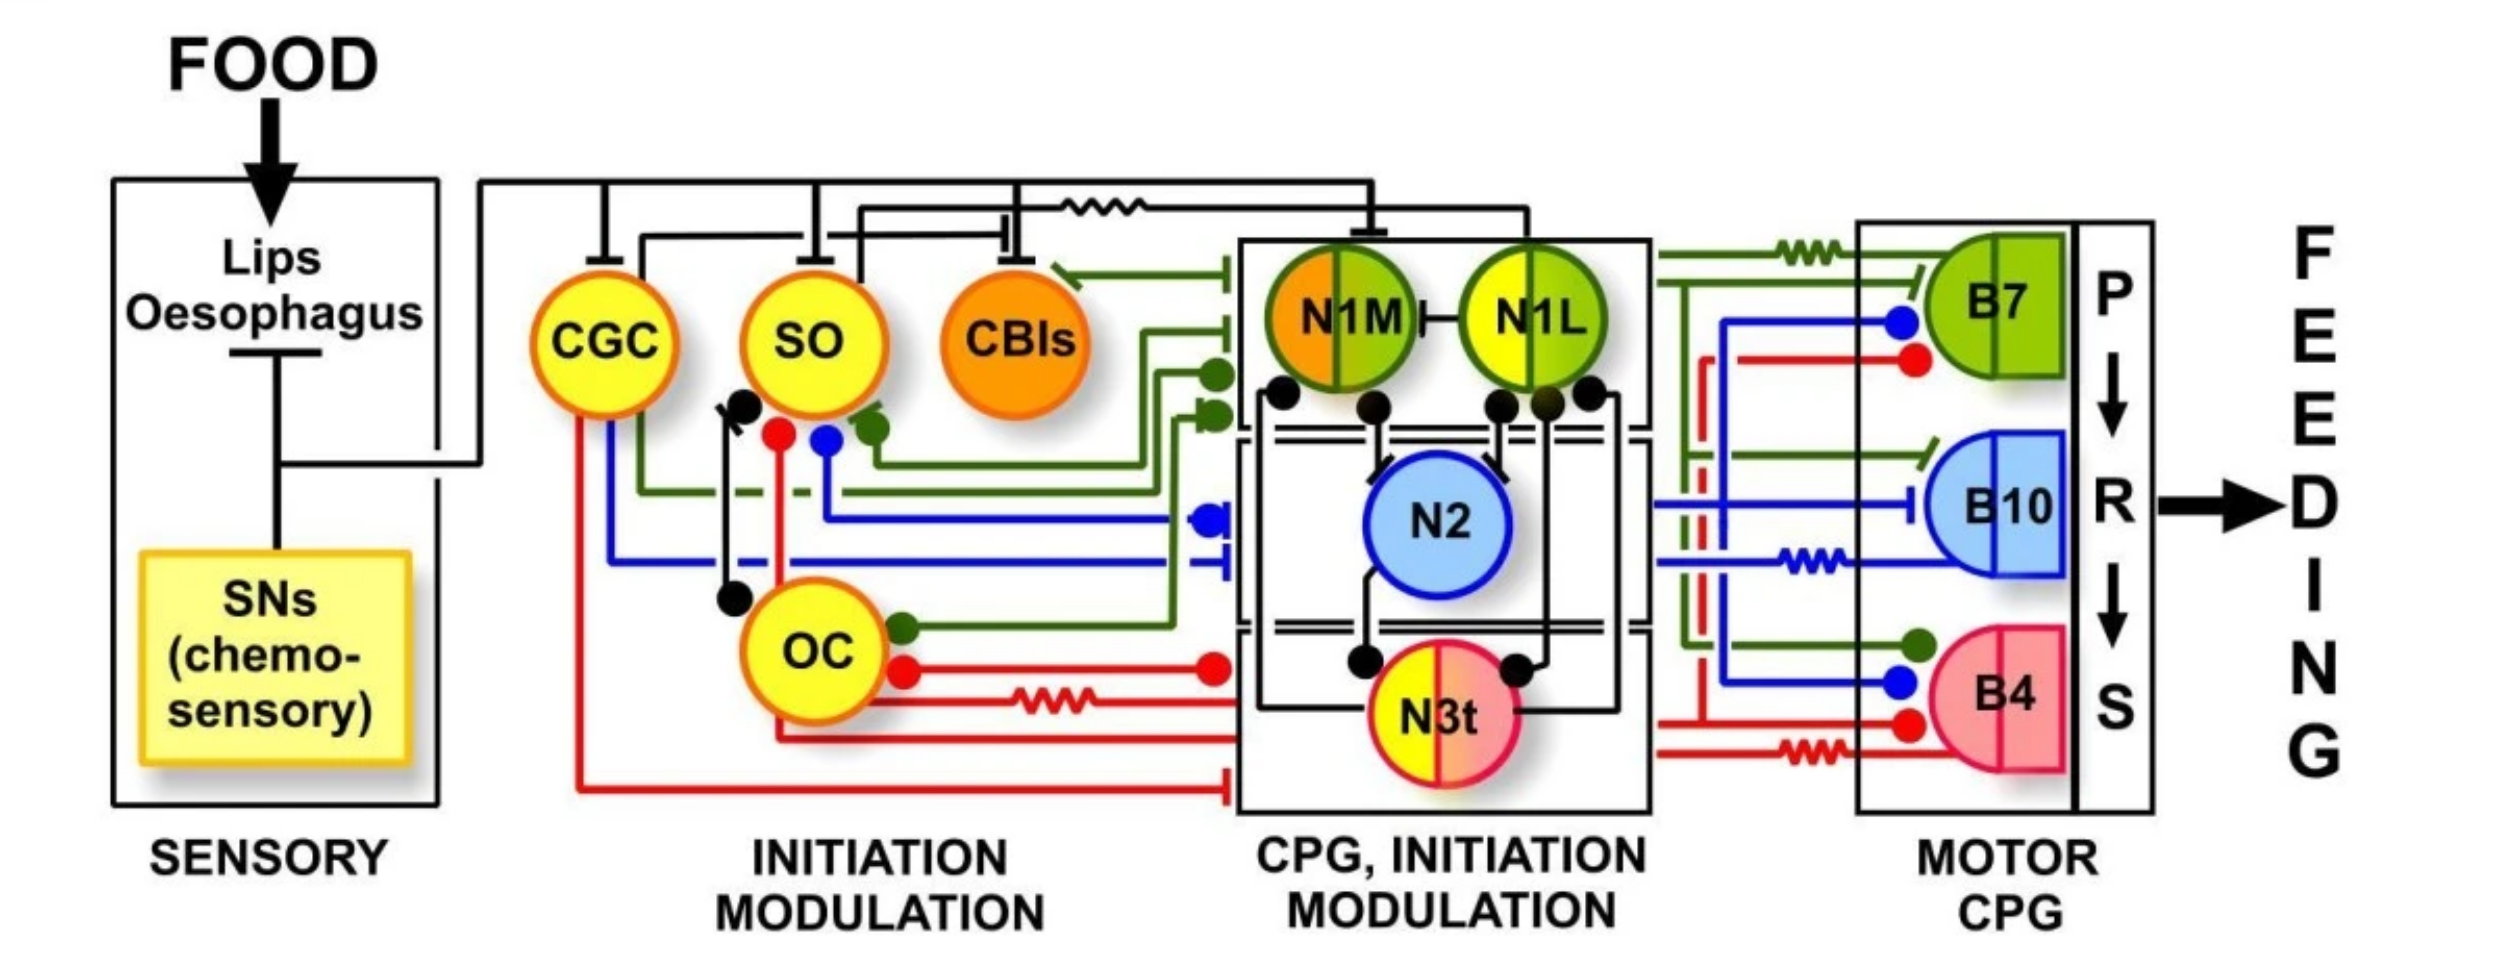
\includegraphics[width=\textwidth]{img/invariants/distributed_benjamin_2012.png}
	\caption{Representation of the distributed system of the feeding CPG. Dots indicate inhibitory chemical synapses, bars excitatory chemical synapses and resistor symbols electrical synapses. Colors indicate the function of the neuron classified as modulatory or initiator (yellow and orange, respectively), and the three phases: protraction, rasp and swallow (green, blue and red, respectively). From left to right: food detection represented by Lips that stimulate CGC, SO CBIs and N1M neurons initiate the rhythm. The ongoing activity is then modulated by those neurons but also by OC neurons and N1 and N3t neurons. Some examples of motoneurons are represented on the right side of the panel, associated to each feeding phase. This figure was adapted from Panel C of Fig. 1 in \textcite{benjamin_distributed_2012} (work under license \href{http://creativecommons.org/licenses/by/2.0}{Creative Commons Attribution}).}
	%	Synaptic connectivity and functions of neurons in the feeding circuit. Modulatory function is indicated by yellow and initiating function by orange. CPG interneurons and motoneurons active during the three phases of the feeding rhythm are indicated by green (P = protraction), blue (R = rasp) and red (S = swallow). Neurons labeled with two colors have two functions. Dots indicate inhibitory chemical synapses, bars excitatory chemical synapses and resistor symbols electrotonic (electrical) synapses. This figure emphasizes the point that many of the neurons have more than function in the feeding network. See Abbreviations for all definitions of neuron types.
	\label{fig:feeding distribution}%
\end{figure}

%Benjamin2012    One of the central controllers of
%spontaneous feeding is the N3t CPG interneuron and
%this cell is involved in mediating the effects of hunger
%and satiety. As was described earlier, the N3ts fire toni-
%cally to inhibit the N1M cells and the rate of this tonic
%activity determines the level of activity in the whole feed-
%ing CPG. By comparing the rates of firing in isolated
%ganglia it was found that the N3t firing frequency was
%higher in satiated compared with starved snails and that
%this was inversely correlated to the frequency of sponta-
%neously fictive feeding cycles [4]. 

%kemenes 2001
%CV1a by modulating motoneuron burst duration and SO by setting the frequency of the ongoing rhythm

In this section we will analyze and describe different examples of experiments for the isolated ganglia with intracellular recordings under different conditions: spontaneous activity, SO-driven activity (spontaneous and by stimulation), medium lip nerve (MLN) stimulation driven activity, and CV1a-driven activity by induced stimulation.

\subsection{Invariants in spontaneous activity}
The spontaneous activity here refers to intracellular recordings of the buccal ganglia after the isolation of the CNS with no chemical or electrical induced stimulation. In that case, since the CPG is able to maintain the activity in an autonomous manner, it keeps the motor activity as if the CNS was not isolated. In this condition, although the characterization of the sequential dynamical invariants can be done, their possible functionality association is more complicated, since the context of the movement origin is lost. The study of these sequential restriction in artificial stimulation contexts can help classify this spontaneous activity, even when the rest of the system is not available. 

Here we analyze three examples of spontaneous activity. We do not know what was the source or context for the feeding activation, but there are differences between the three experiments regarding their dynamical invariants. The case with the strongest linear correlation is the first example shown in Fig. \ref{fig:prep2 invariants}, where the N3 burst duration and the associated intervals covering N3 phase (N2N1 interval, N3N1 interval, N3N2 interval and N2N1 delay) had a strong linear correlation with the period ($R^2 > 0.9$). This is also clear in the variability boxplot, where the variability distribution of the period is really similar to that of N3 burst duration, N2N1 interval, N3N1 interval, N3N2 interval and N2N1 delay, and the rest of the intervals are not similar to the period. This difference in variability is also important, since while there are intervals with a strong linear correlations illustrating cycle-by-cycle dynamical restrictions, some other intervals have no relation, all have $R^2 < 0.1$, i.e., are free to display unrelated variability. Observing the recording of this example (first row in Fig. \ref{fig:prep2 invariants}), we can see that the N3 neuron had long periods of tonic firing (which were excluded from the time-interval relations), and that the spontaneous activity was lead by N3 neuron, associated in the literature with spontaneous activity in satiated animals. The N3t was tonically firing producing long periods of silence interrupted by short rasps \parencite{staras_loss_2003,benjamin_distributed_2012}.

In the following examples shown in Figs. \ref{fig:prep3 invariants} and \ref{fig:prep1 invariants}, the variability distribution is different. In the example shown in Fig. \ref{fig:prep3 invariants}, we can see the distribution of the variability between N1 and N3 phases illustrated in the boxplot and also in the linear regressions, in which, although they have low $R^2$ values, we can observe some linear tendencies between specific time intervals and the period, specially in combined intervals such as the N3-N2 interval. A common characteristic with the previous example is the presence of unrelated intervals to the period, since N2 burst durations and other time-intervals associated to the N2 phase (N2N3 delay, N1N2 delay) have $R^2 < 0.1$. These intervals also remain unrelated to the period in the third example, shown in Fig. \ref{fig:prep1 invariants}, where N2 and N2N3 delay have similar $R^2$ values. In that last case, however, the variability is mostly in the N1 phase. Again, the linear correlations with the period are in combined periods, usually the ones involving N1 and N3 phases: N31N1 interval, N2N1 delay, N3N1 delay; this points to the distribution of variability between those two phases. Also, the fact that the combined intervals have much stronger linear correlations is affected by the time references in these intervals.

%Since the first and last spike of the burst are not always well-defined, intervals like the delay give us more information than in the model study described in the previous section \ref{sec:CPG model equations equations}.

%In the absence of food, particularly in satiated animals (see the Hunger and satiety section, below), snails show long periods of quiescence with only occasional spontaneous rasps. It has been shown that the quiescence is due to tonic inhibition of the N1Ms by the N3ts [4]. During quiescence the N3ts fire continuously and via the strong inhibitory connection prevent N1M plateauing (Figure 4B, left). When sucrose is applied to the lips (Figure 4A), the N3ts are hyperpolarized (Figure 4C) reducing the level of tonic inhibition to the N1M and this has a permissive effect in allowing the N1M to plateau (Figure 4C). Thus during the sucrose-driven feeding pattern, the N3ts fire rhythmically as part of the feeding CPG (Figure 4B, right) due to the reciprocal inhibitory synaptic connections with the N1Ms. Thus N3ts have a role in modulating the feeding network as well as being part of the CPG (Figure 1C).


\begin{figure}[htbp]
	\centering
	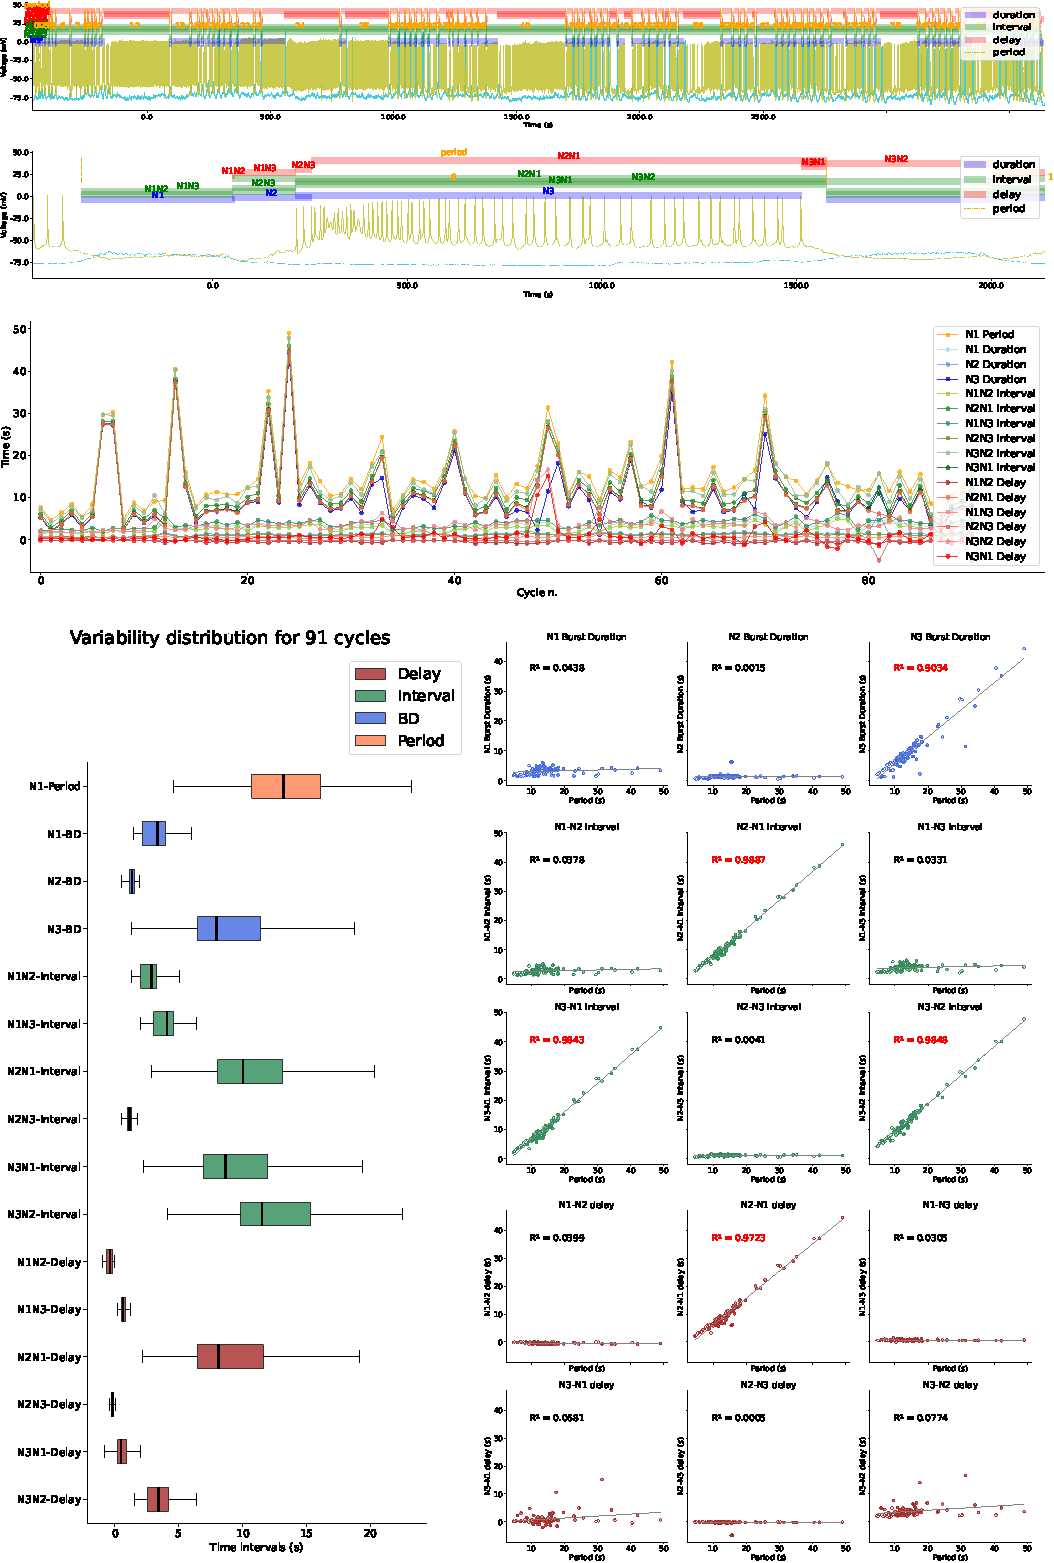
\includegraphics[width=0.9\textwidth]{./img/invariants/data/SUSSEX/prep2/images/3phases/panel_with_intervals.pdf}
	\caption{\textbf{Spontaneous case 1}: Panel of interval distributions and dynamical invariants for the three phases in the CPG for spontaneous activity. a) Voltage traces for the intracellular recording analyzed for this panel. b) Representation of the time-intervals described. c) Duration of each time interval ($y-axis$) at each cycle. d) Box-plot with the variability distribution of the duration of each time-interval. e) Time-intervals duration against the period for NX-duration (blue), NXNY-Interval (green) and NXNY-Delay (red).}
	\label{fig:prep2 invariants}
\end{figure}

\begin{figure}[htbp]
	\centering
	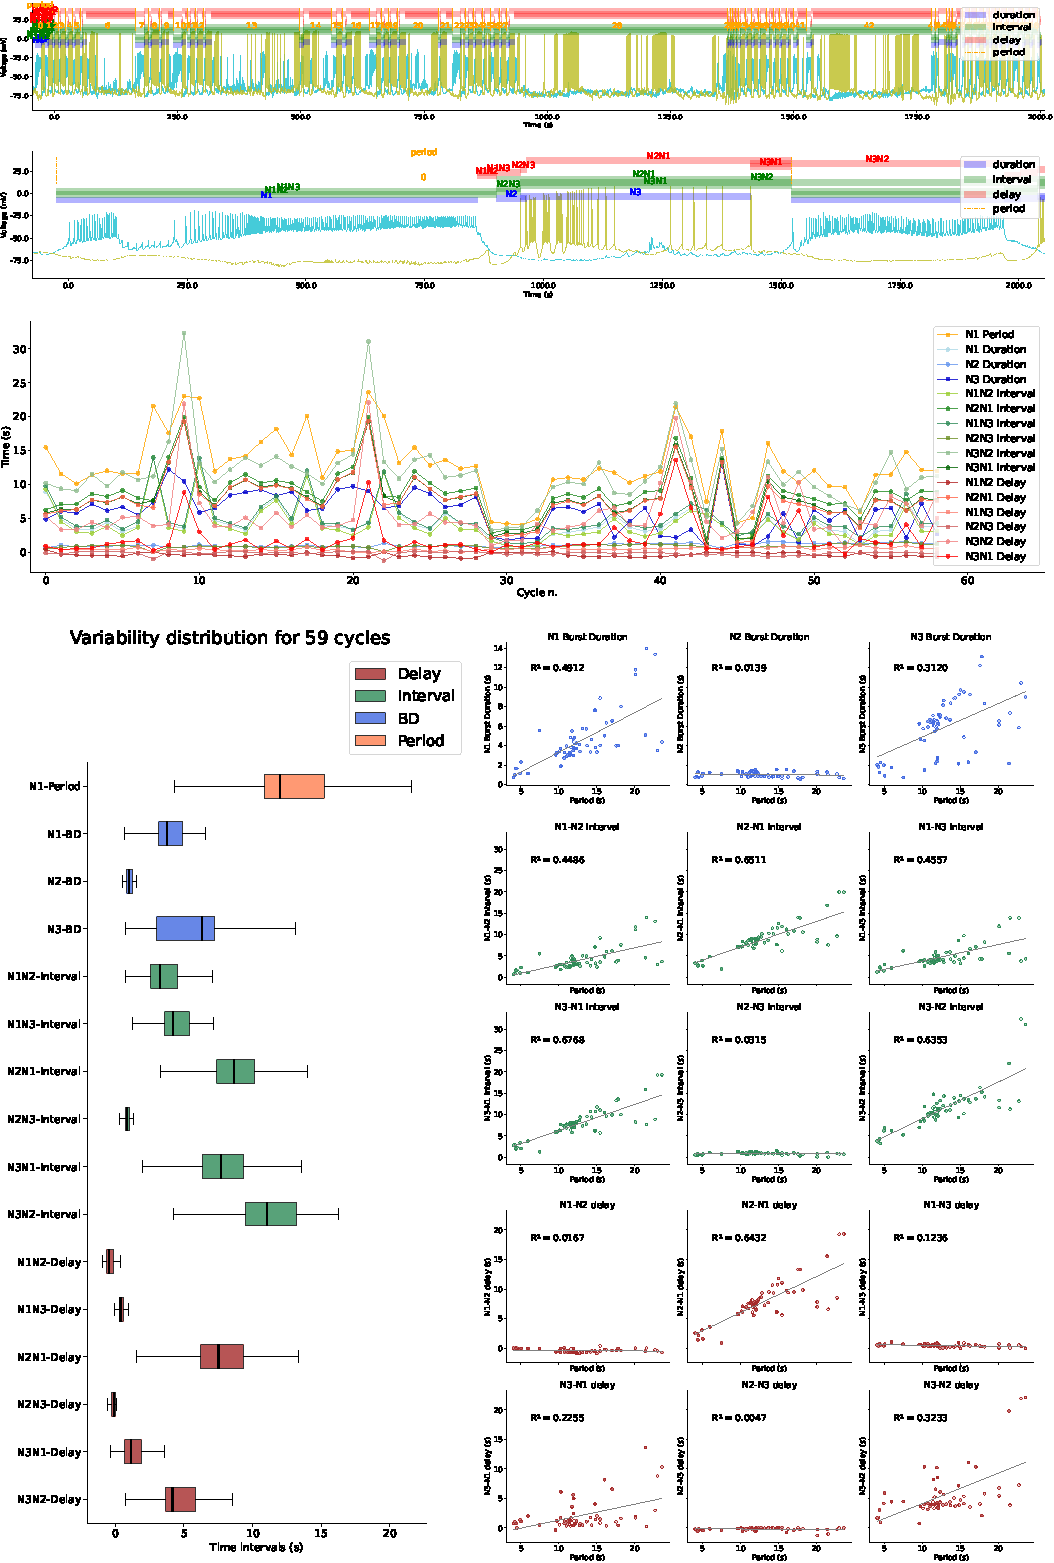
\includegraphics[width=0.9\textwidth]{./img/invariants/data/SUSSEX/prep3/images/3phases/panel_with_intervals.pdf}
	\caption{\textbf{Spontaneous case 2}: Panel of interval distributions and dynamical invariants for the three phases in the CPG for spontaneous activity. a) Voltage traces for the intracellular recording analyzed for this panel. b) Representation of the time-intervals described. c) Duration of each time interval ($y-axis$) at each cycle. d) Box-plot with the variability distribution of the duration of each time-interval. e) Time-intervals duration against the period for NX-duration (blue), NXNY-Interval (green) and NXNY-Delay (red).}
	\label{fig:prep3 invariants}
\end{figure}

\begin{figure}[htbp]
	\centering
	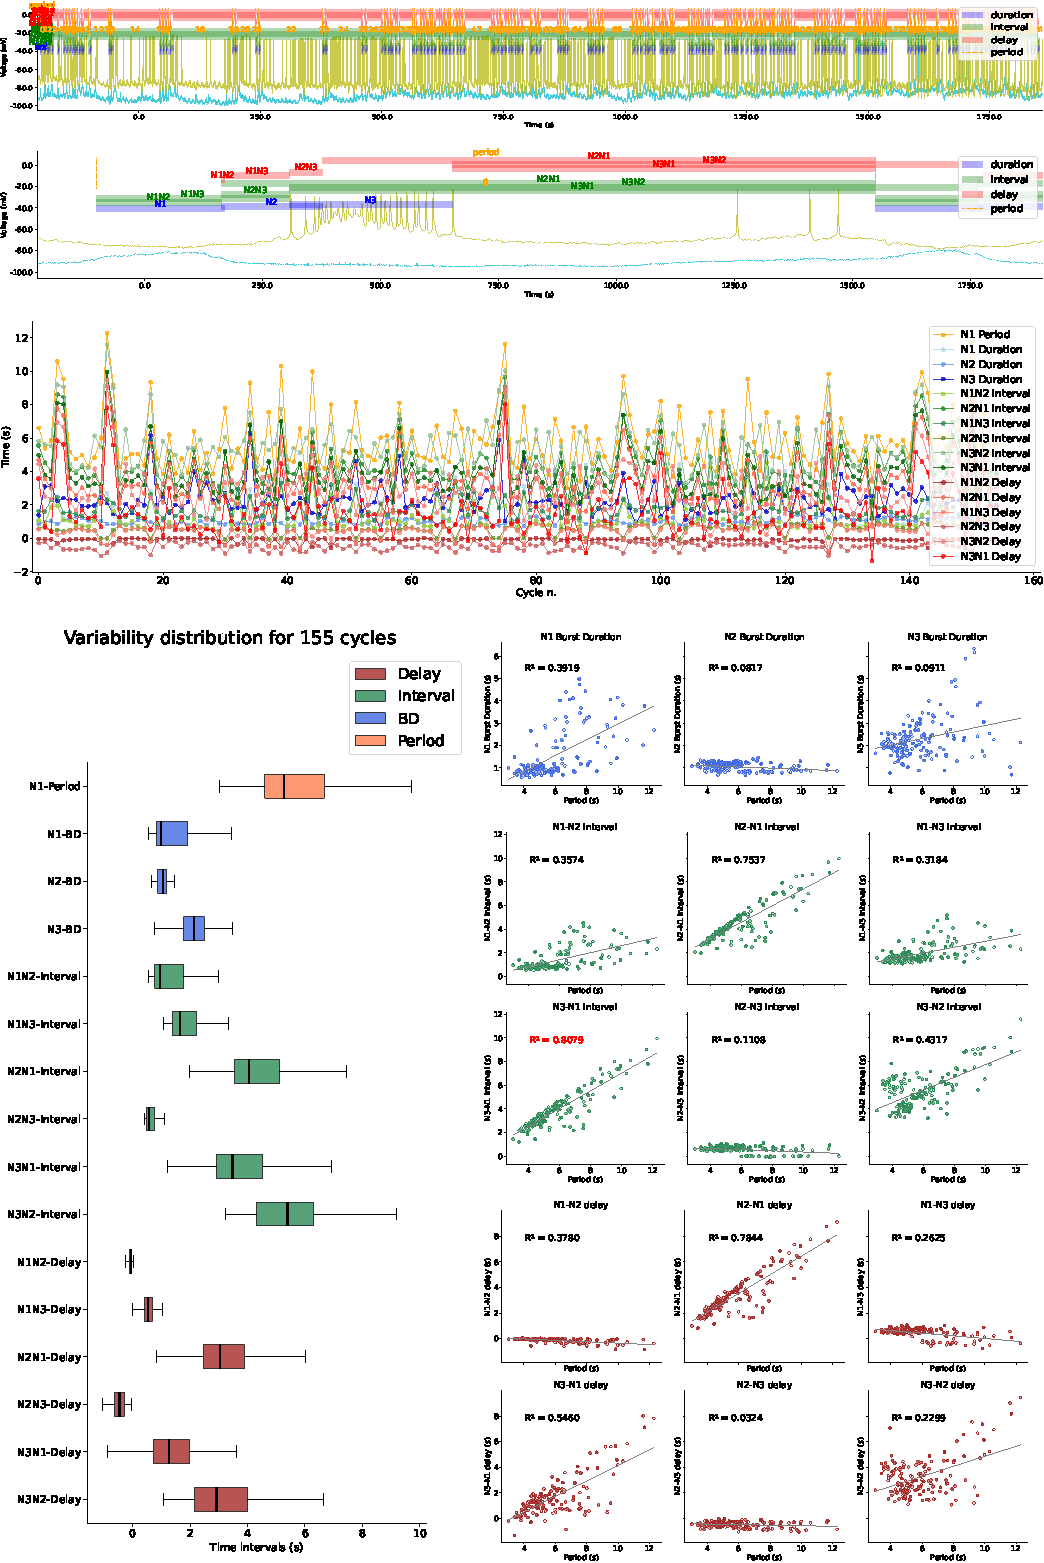
\includegraphics[width=0.9\textwidth]{./img/invariants/data/SUSSEX/prep1/images/3phases/panel_with_intervals.pdf}
	\caption{\textbf{Spontaneous case 3}: Panel of interval distributions and dynamical invariants for the three phases in the CPG for spontaneous activity. a) Voltage traces for the intracellular recording analyzed for this panel. b) Representation of the time-intervals described. c) Duration of each time interval ($y-axis$) at each cycle. d) Box-plot with the variability distribution of the duration of each time-interval. e) Time-intervals duration against the period for NX-duration (blue), NXNY-Interval (green) and NXNY-Delay (red).}
	\label{fig:prep1 invariants}
\end{figure}


Figure \ref{fig:spontaneous pairplot comparison} shows the pairplots for each of these three experiments, with all possible combinations between intervals. Note that, for a better representation, there are only two phases taken here into account: N1 and N3. (Figures \ref{fig:prep2 invariants pairplot}, \ref{fig:prep3 invariants pairplot} and \ref{fig:prep1 invariants pairplot} in the Appendix show the pairplot for intervals from the three-phases). Most part of the time-intervals involved in the N2 phase are contained in the N1N3 delay, which goes from the end of N1 to the start of N3 (see \ref{subsec:intervals}). The intervals' relations with the period correspond to the first column, the rest are combinations between all possible intervals, including the period defined from N3 start to N3 end. We see again that each recording has a different variability distribution: In the first panel, we can observe several robust dynamical invariants. This is also the case for the second panel, where we can observe that, in relation to N1 and N3, it is interesting to see that the N1-BD has a really strong linear relation with the N1N3 interval, which suggests that all variability in that phase comes from the burst duration, and the N2 phase remains mostly constant. In the last panel, we can appreciate this increase in the correlation between N1-BD and the period and the decrease in the correlation with the N3-BD. This is shown in the linear correlation unveiled in this pairplot by the N3N1-Interval and the N3N1-Delay, representing the constancy in the time duration of the burst.  

\begin{figure}[htbp]
	\centering
	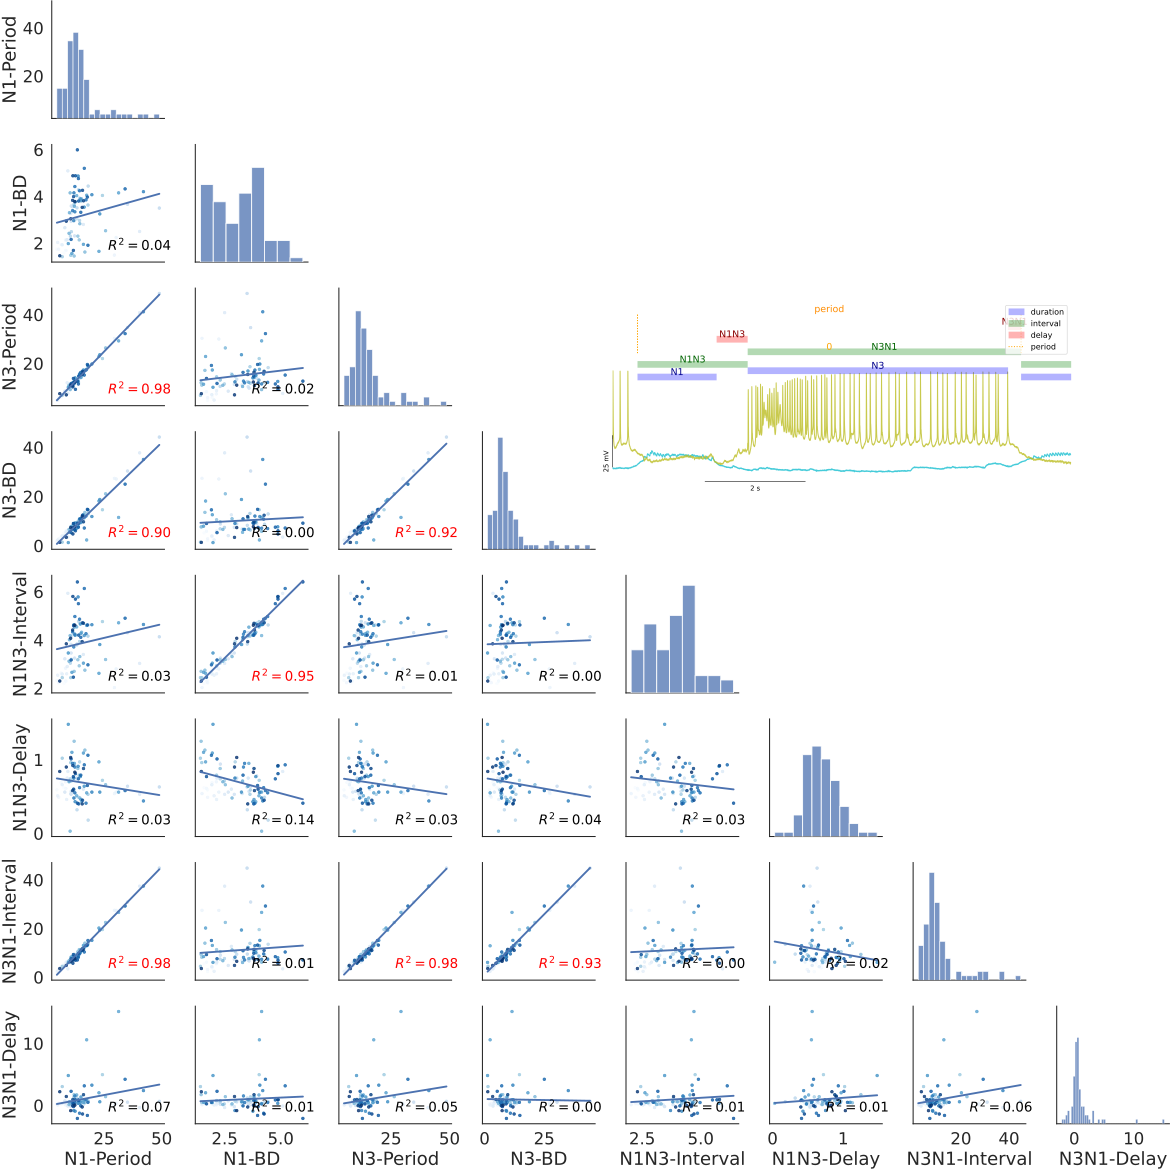
\includegraphics[width=0.48\textwidth]{./img/invariants/data/SUSSEX/prep2/images/2phases/panel_with_pairplot.png}
	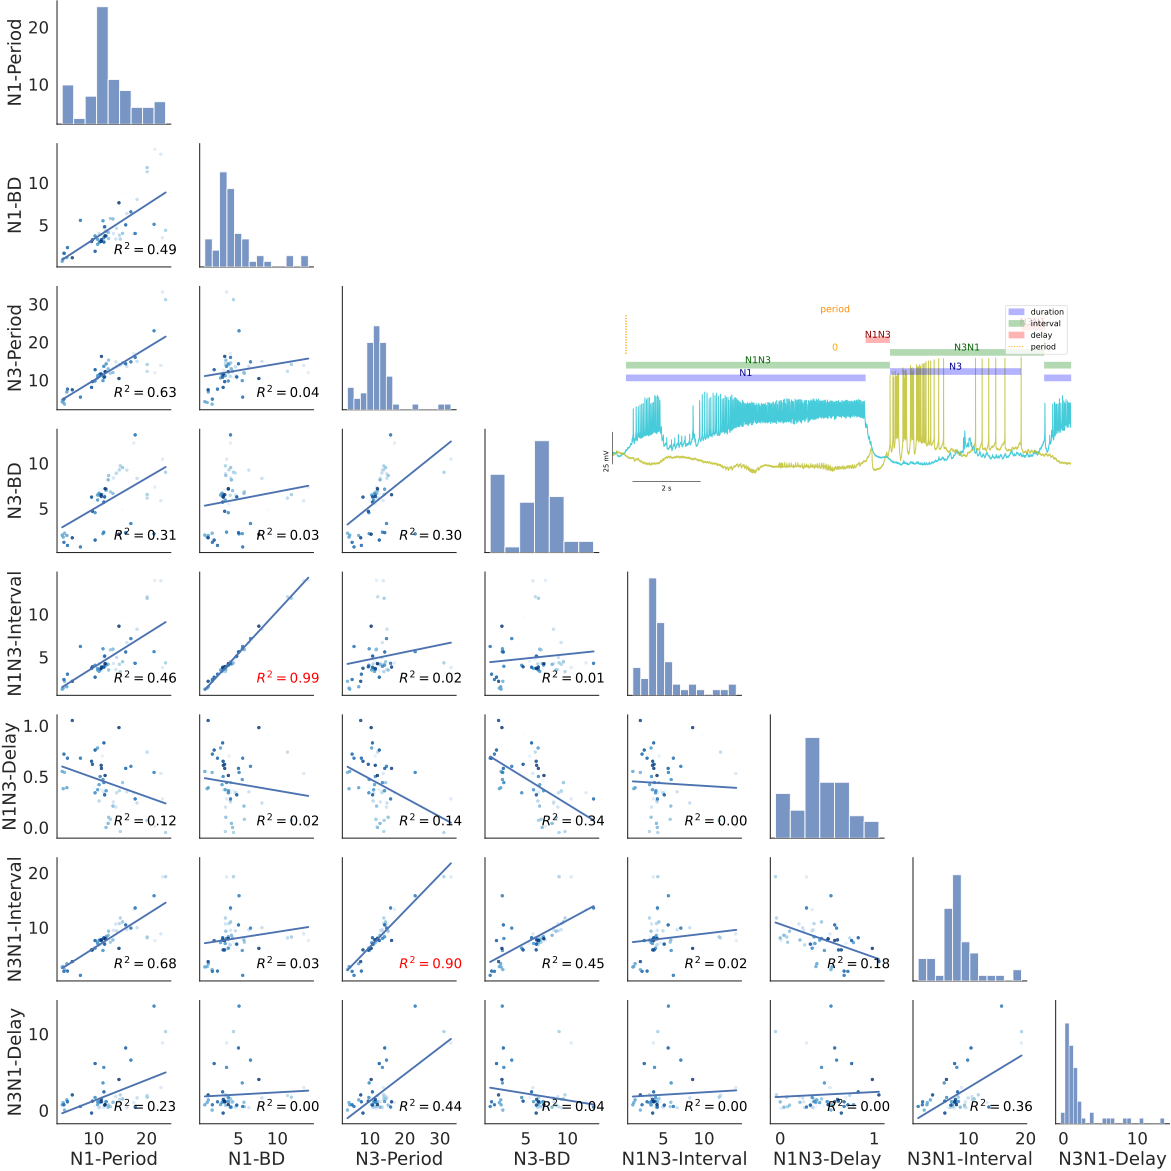
\includegraphics[width=0.48\textwidth]{./img/invariants/data/SUSSEX/prep3/images/2phases/panel_with_pairplot.png}
	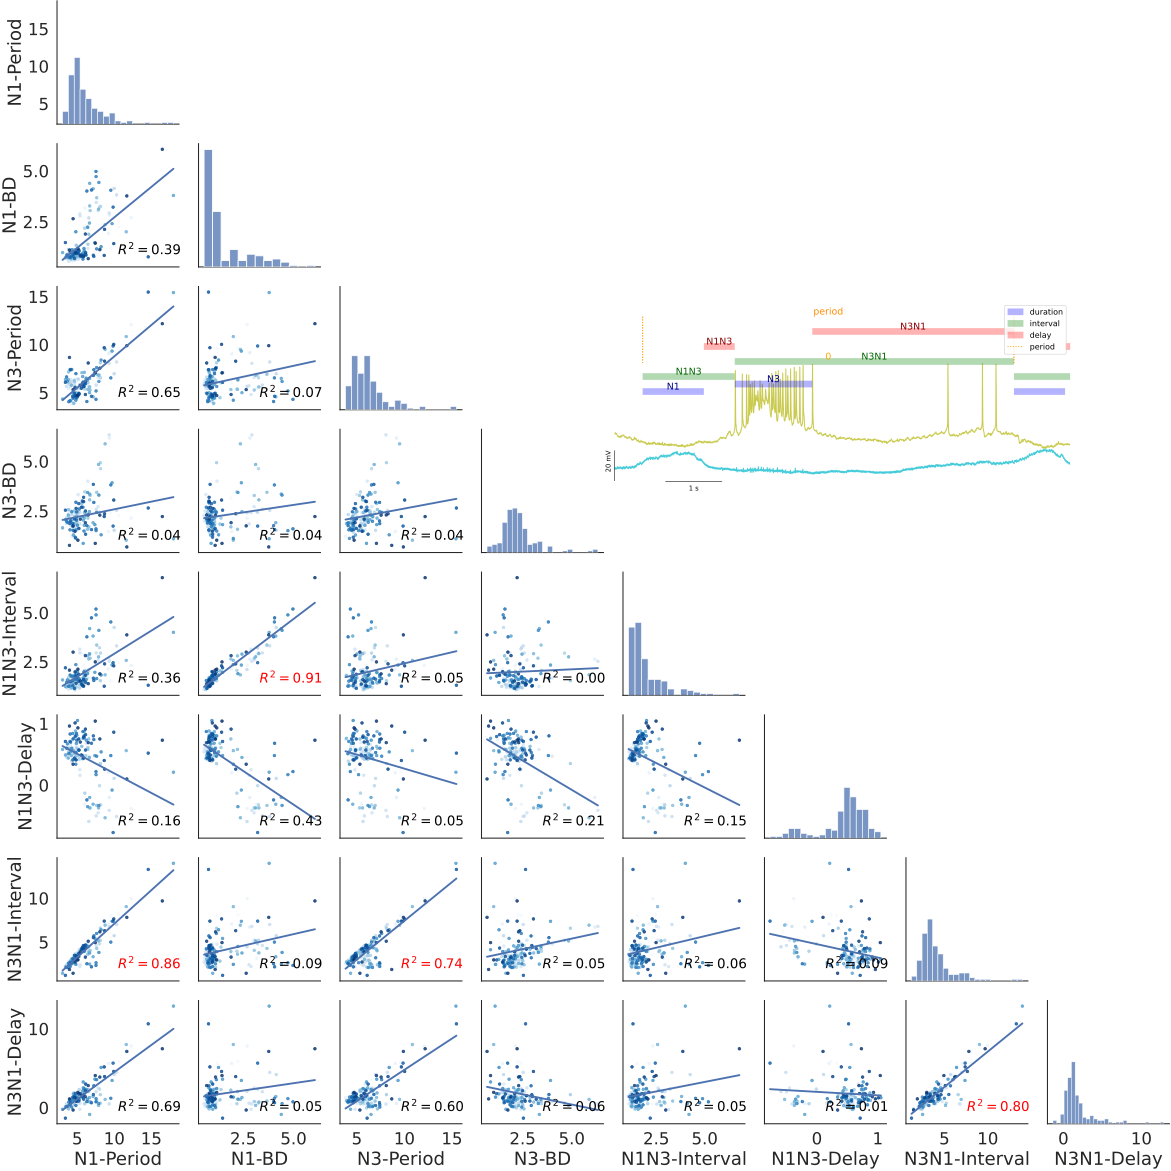
\includegraphics[width=0.48\textwidth]{./img/invariants/data/SUSSEX/prep1/images/2phases/panel_with_pairplot.png}
	\caption{Spontaneous activity summary: Panel of the pairplots for all possible combinations between the time intervals defined for two phases (N1 and N3) in the CPG recordings for the three examples of spontaneous activity recordings.}
	\label{fig:spontaneous pairplot comparison}
\end{figure}


\clearpage
\newpage
\subsection{Invariants in SO driven activity}
As we saw before, the SO role in the feeding CPG is modulatory, which means, that it modifies the rhythm once it is activated. In the model analysis, in section \ref{subsec:so driven}, we showed that when the variability in the simulations was induced by adding a ramp current to the SO neuron, the time-interval variability was distributed between the N1 and N3 phases, having both a strong correlation with the period, which increased the $R^2$ values. Therefore, in the living recordings we can expect that the variability cycle-by-cycle is distributed during the modulation of SO, which is connected to N1M and N3t (see Fig. \ref{fig:feeding distribution}). 

In this subsection, we will see an example from a spontaneous activity where the SO neuron was modulating for two lapses of time during the recording. This can be identified by the inhibition of B4 and the activation of B3, as illustrated in Fig. \ref{fig:SO-spontaneous-driven}. We can also see in this figure how, during the SO modulation, the rhythm was "stabilized" with less variability in the intervals' duration. The characterization of the variability of the time intervals and their relation to the cycle period for this trace is depicted in Figs. \ref{fig:so spontaneous invariants 1},\ref{fig:no so spontaneous invariants} and \ref{fig:so spontaneous invariants 2}, when SO was modulating, when it ceased its modulation, and when it then restarted it, respectively. 


 \begin{figure}[htbp]
 	\centering
 	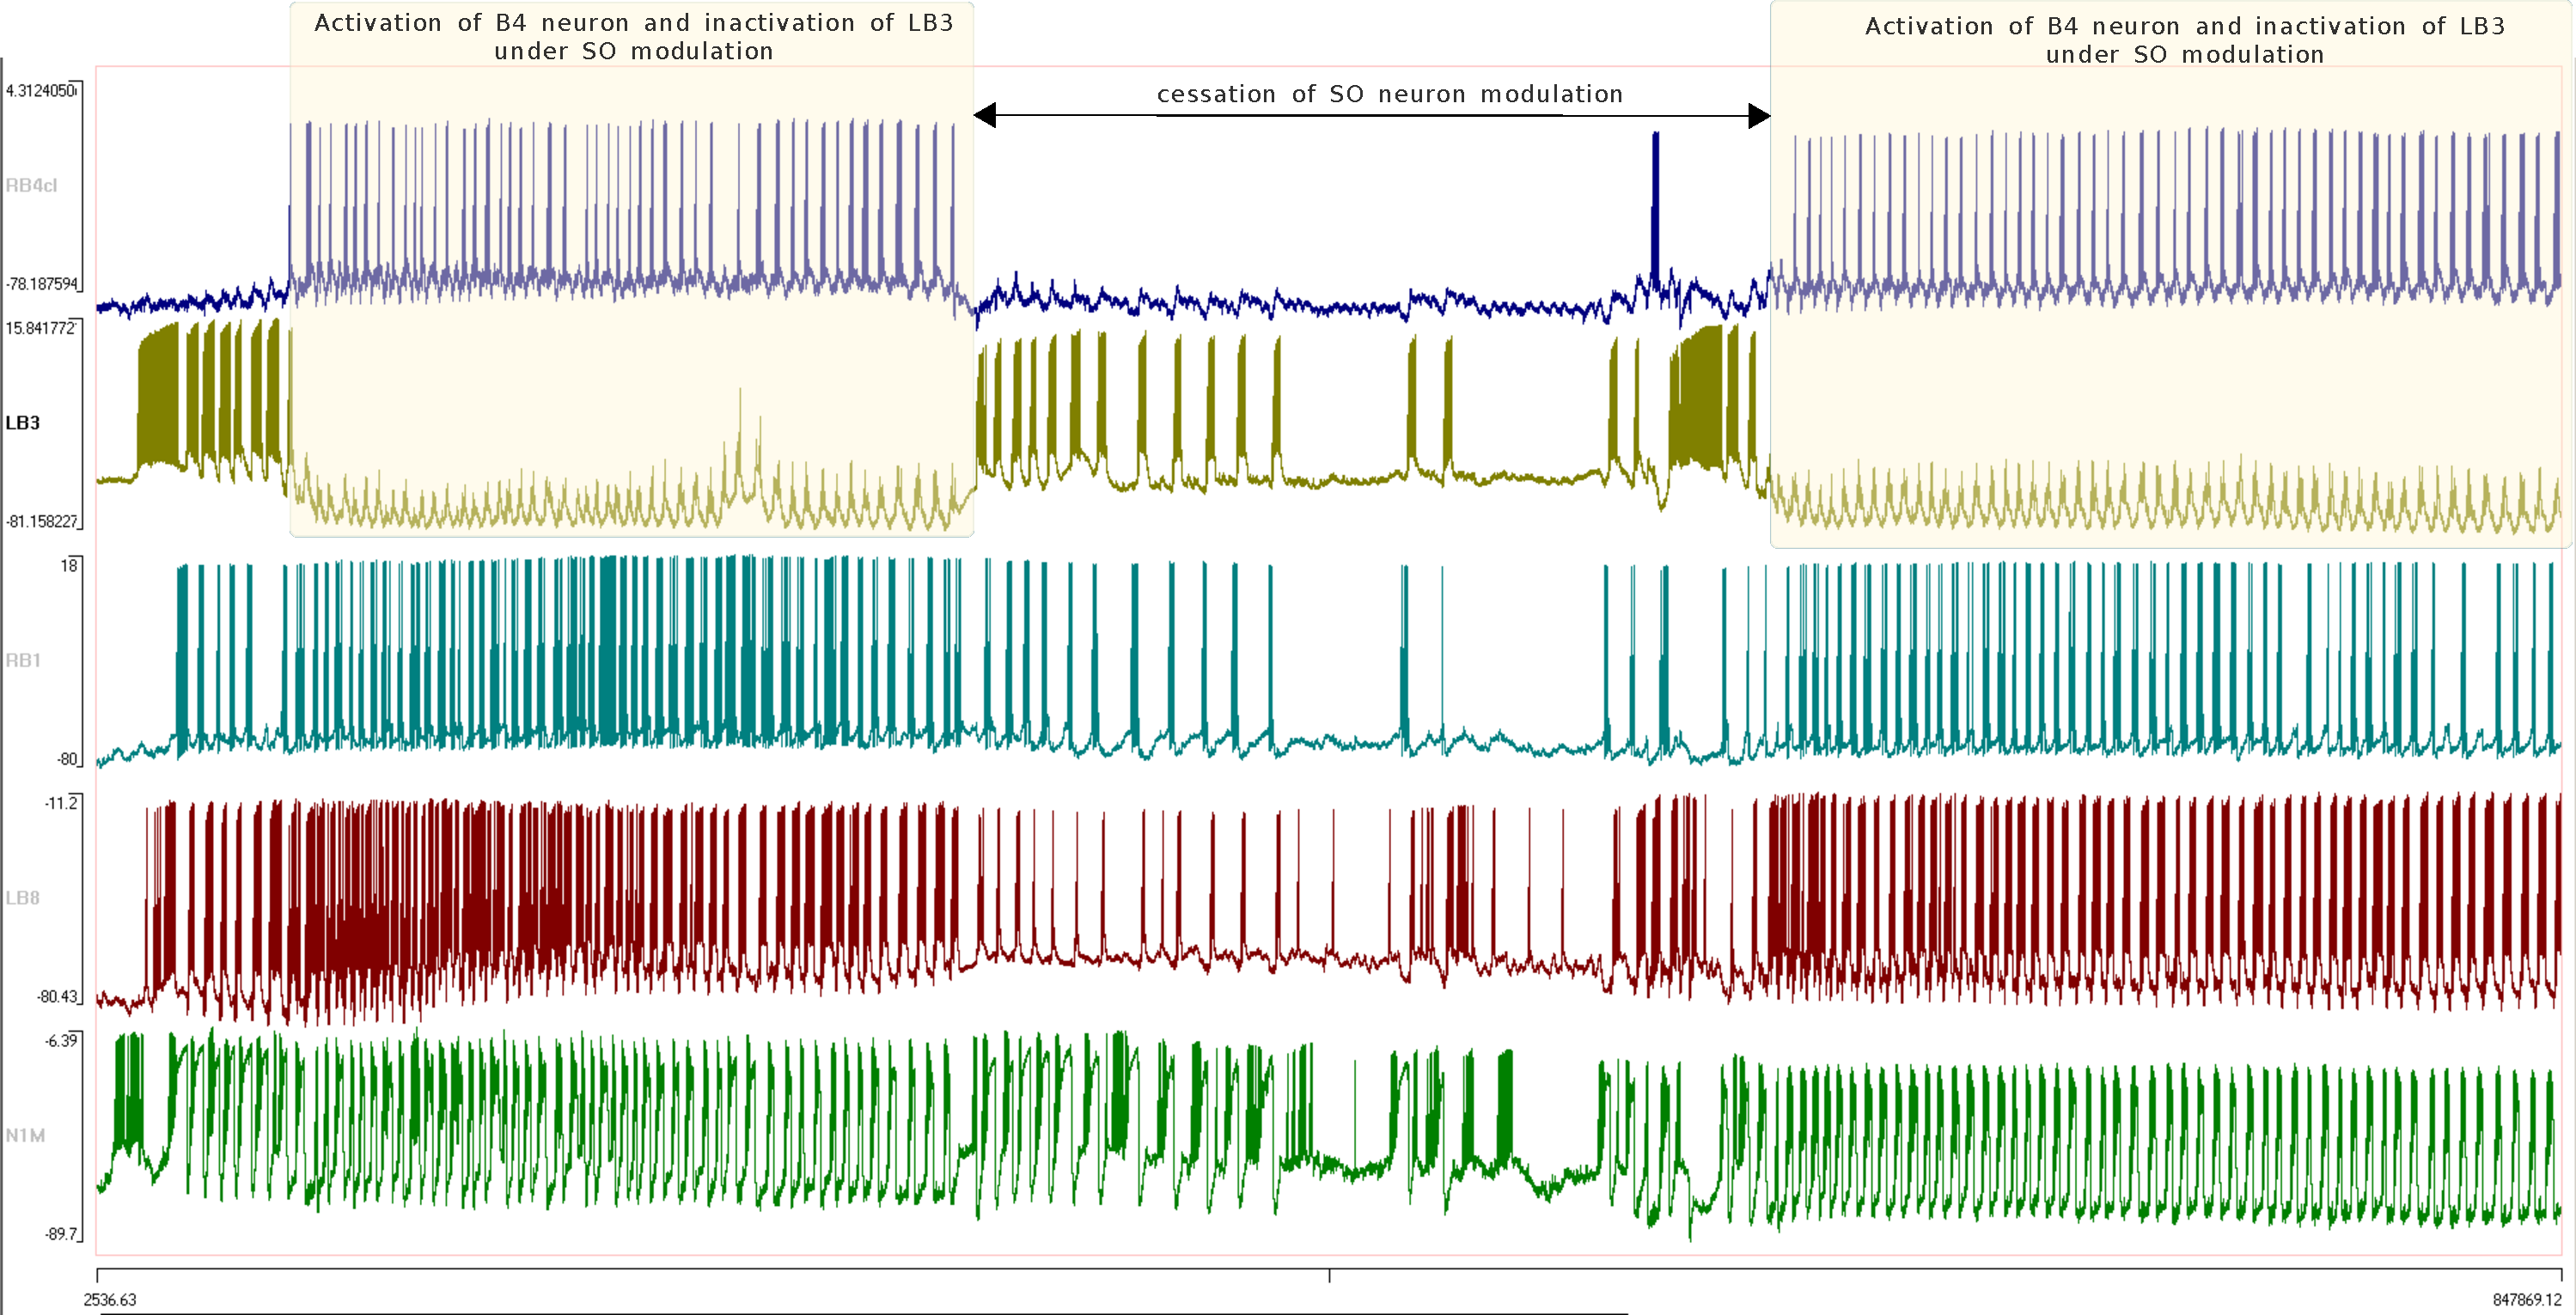
\includegraphics[width=\textwidth]{./img/invariants/SO-spontaneuous-driven.pdf}
 	\caption{Representation of recordings of the spontaneous activity with lapses of SO modulation. The parts of the recording with yellow background highlight when the activity was modulated by the SO neuron. From top to bottom: intracellular recording of a neuron from the B4 cluster, B3 motoneuron, B1 motoneuron, B8 motoneuron, and N1M interneuron.}
 	\label{fig:SO-spontaneous-driven}
 \end{figure}

When the rhythm was driven by SO, we can see how the variability for N1-BD and N3-BD was limited, which is  reflected in the low variability observed in the boxplots of Figs. \ref{fig:so spontaneous invariants 1} and \ref{fig:so spontaneous invariants 2}, and also panels c) for both cases that show the duration of each interval per cycle and there were not large changes in the duration, as we saw for example in Fig. \ref{fig:prep2 invariants}.c). In the correlation of the intervals with the period, shown in panel e), although $R^2$ value is not significantly high, N1-BD and N3-BD have around 0.7 and 0.3 in both cases, pointing to this redistribution of the variability. Figure \ref{fig:no so spontaneous invariants} shows the characterization of the intervals variability when the SO stops its modulation. During that lapse of time (depicted in Fig. \ref{fig:SO-spontaneous-driven}), the variability concentrates in the N1 phase as it can be seen in the duration of the interval in panels c) and d), and also in the high correlation to the period in panel e) only for intervals such as N1-BD ($R^2=0.9$). Also, while the $R^2$ value of N1-BD is in the order of 0.9, the N3-BD is close to 0. Although this example had only a few cycles, it suggests that the variability in that lapse of time was all carried by the N1 phase. Regarding the rest of the time-intervals in the cycle, the one with the largest variability is N3N1 interval, since it contains N1-BD. Also, when activity ceases, the N3N1 delay variability rises, which is notable compared to the rest of the experiments and the model, and might be caused by the burst shape and how the intervals where defined (see Fig. \ref{fig:no so spontaneous invariants}, first panel). This result, also matches the experimental work by \textcite{elliott_temporal_1991}, which showed this distribution between N1-BD and N3-BD. In that work, the SO modulation was induced by stimulating SO neuron. Figure \ref{fig:so induced invariants} shows an example inducing the SO modulation by electrical stimulation. Again, we can see the same variability distribution between N1 and N3 phases, having N1 a strongest correlation with the period, reaching $R^2=0.8$ this time. It is also important to highlight that the intervals associated to N2 phase (N1N3 delay and N3N1 delay) do not have any relation with the period, and their variability is minimal. To further compare this two panels, the pairplots for one example of spontaneous activity and the SO induced modulation are shown in Fig. \ref{fig:so pairplot comparison}. In the pairplot, we see the same interval relations and also another strong relation between N1N3 Interval and N1-BD, which appears in both cases and supports the N1 variability and the constancy of N2 phase, since in the N1N3 interval, all the variability is associated with N1-BD. 

%Acabar comparación con el otro. 
 
\begin{figure}[htbp]
	\centering
	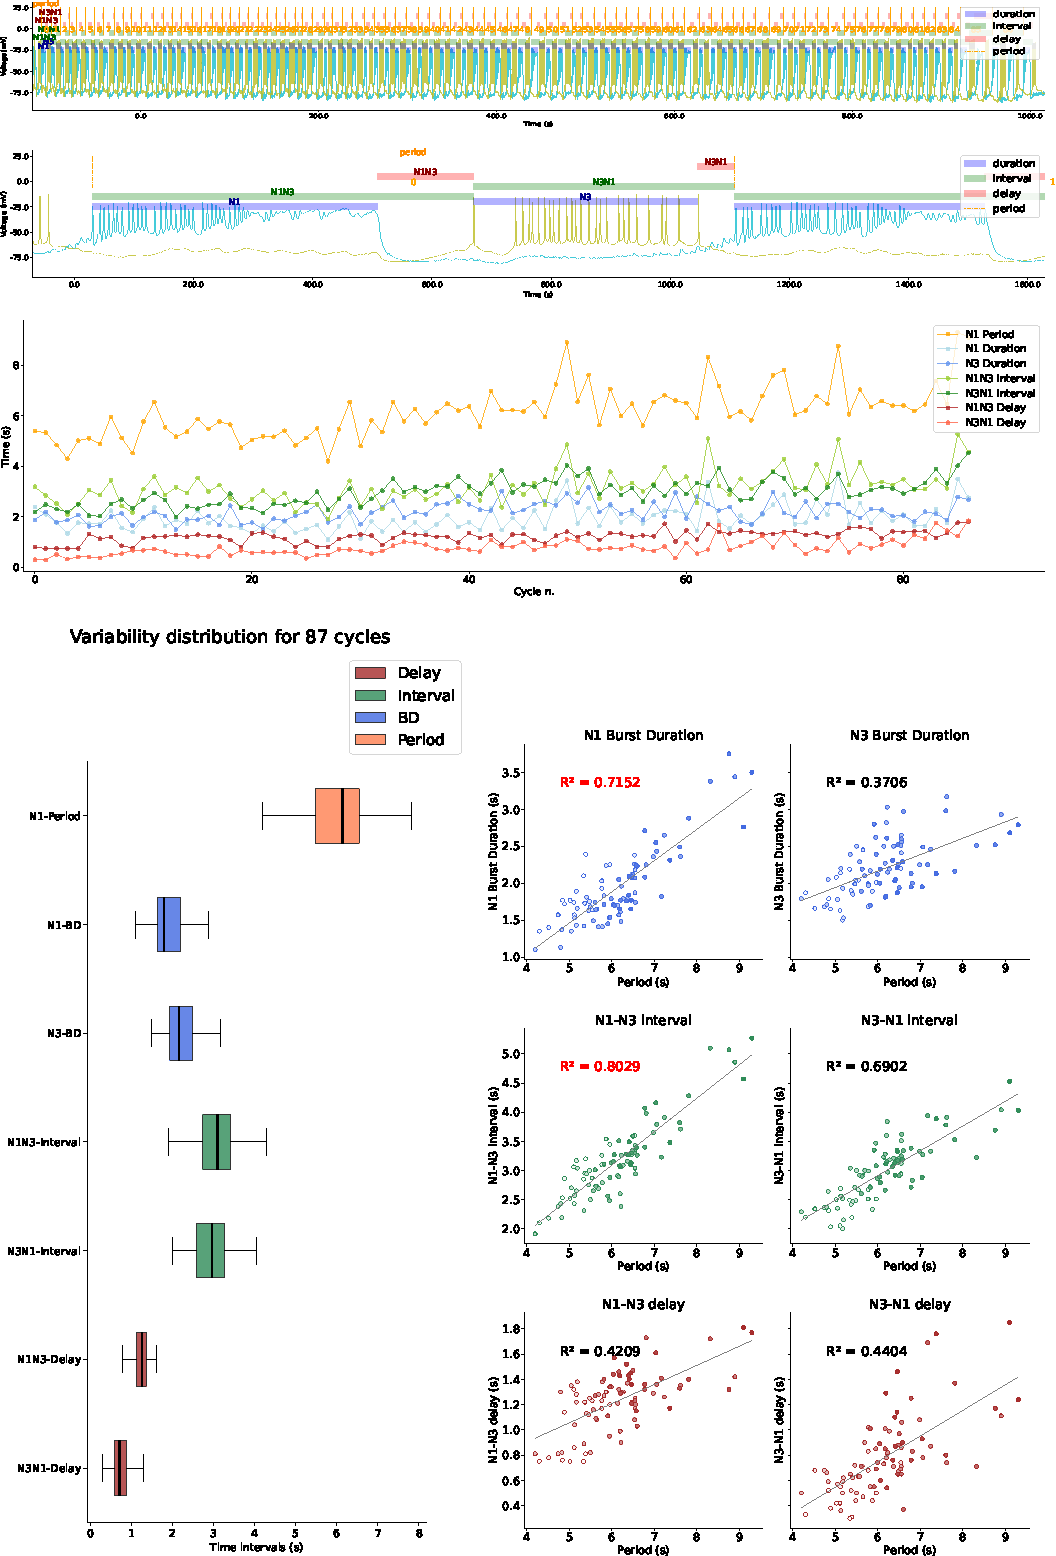
\includegraphics[width=0.9\textwidth]{./img/invariants/data/SUSSEX/prep4_so_driven_2/images/panel_with_intervals.pdf}
	\caption{\textbf{SO neuron driven spontaneous activity}: Panel of interval distributions and dynamical invariants for the two phases in the CPG for spontaneous activity driven by SO neuron. a) Voltage traces for the intracellular recording analyzed for this panel. b) Representation of the time-intervals described. c) Duration of each time interval ($y-axis$) at each cycle. d) Box-plot with the variability distribution of the duration of each time-interval. e) Time-intervals duration against the period for NX-duration (blue), NXNY-Interval (green) and NXNY-Delay (red).}
	\label{fig:so spontaneous invariants 2}
\end{figure}


\begin{figure}[htbp]
	\centering
	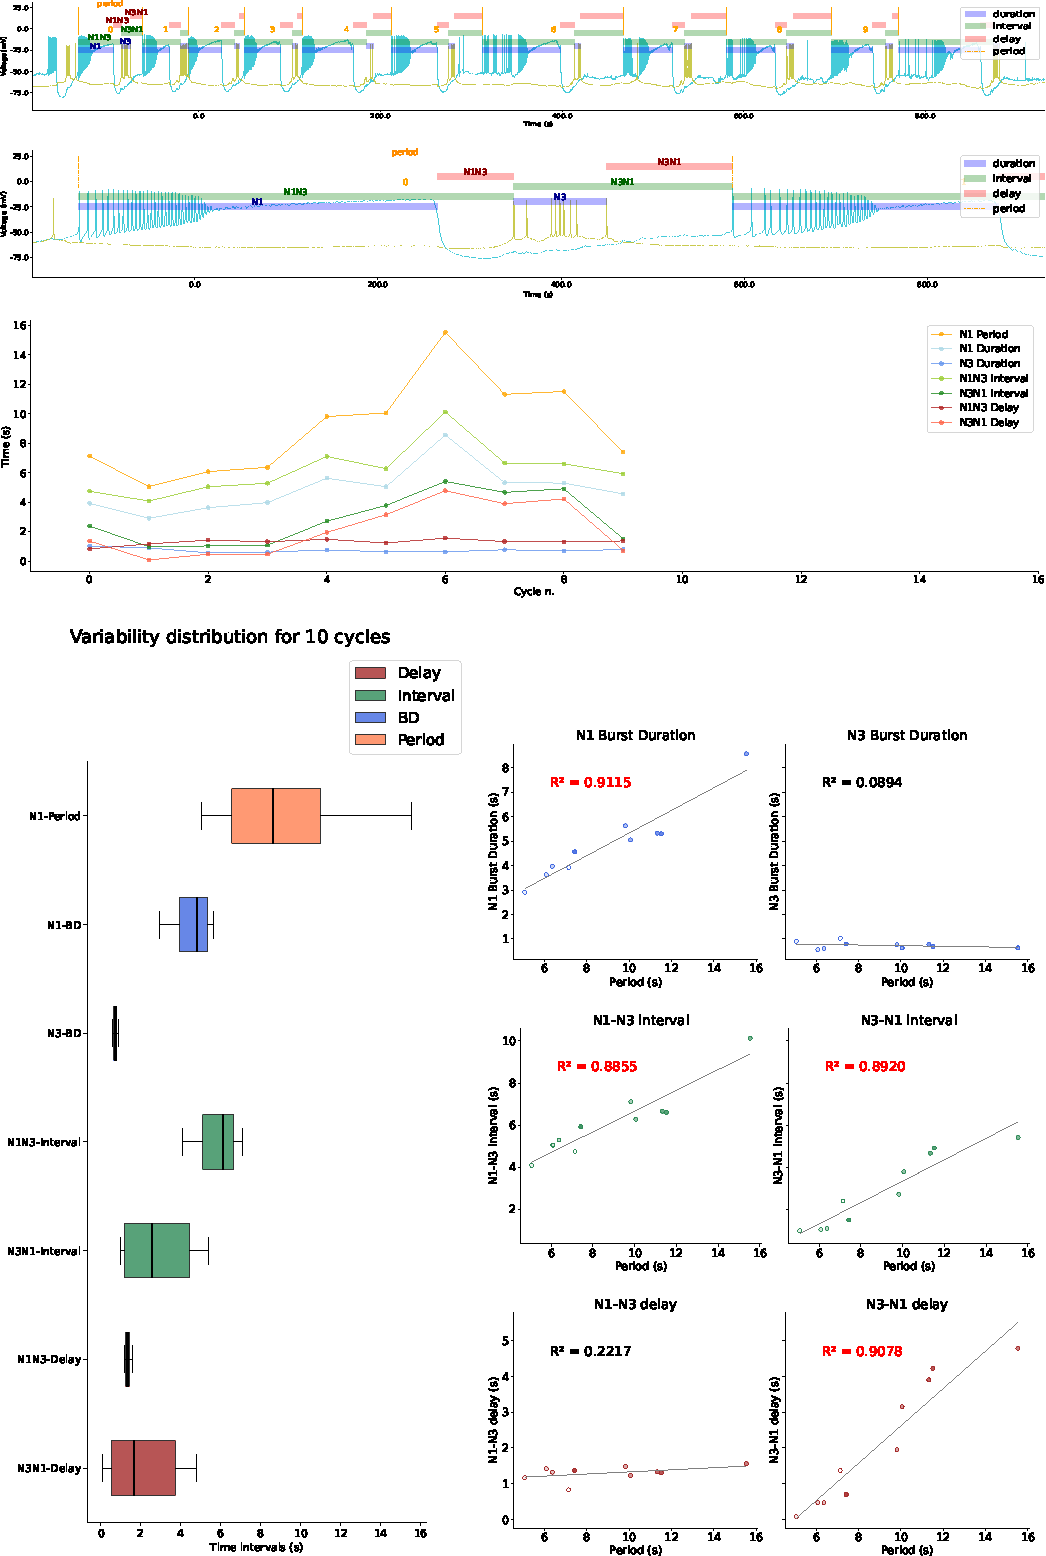
\includegraphics[width=0.9\textwidth]{./img/invariants/data/SUSSEX/prep4_so_no_driven/images/panel_with_intervals.pdf}
	\caption{\textbf{Spontaneous activity when the SO-driven modulation ceases}: Panels illustrate the interval distribution and dynamical invariants for the two phases in the CPG during spontaneous activity without SO modulating the rhythm. a) Voltage traces for the intracellular recording analyzed for this panel. b) Representation of the time-intervals described. c) Duration of each time interval ($y-axis$) at each cycle. d) Box-plot with the variability distribution of the duration of each time-interval. e) Time-intervals duration against the period for NX-duration (blue), NXNY-Interval (green) and NXNY-Delay (red).}
	\label{fig:no so spontaneous invariants}
\end{figure}
 

\begin{figure}[htbp]
	\centering
	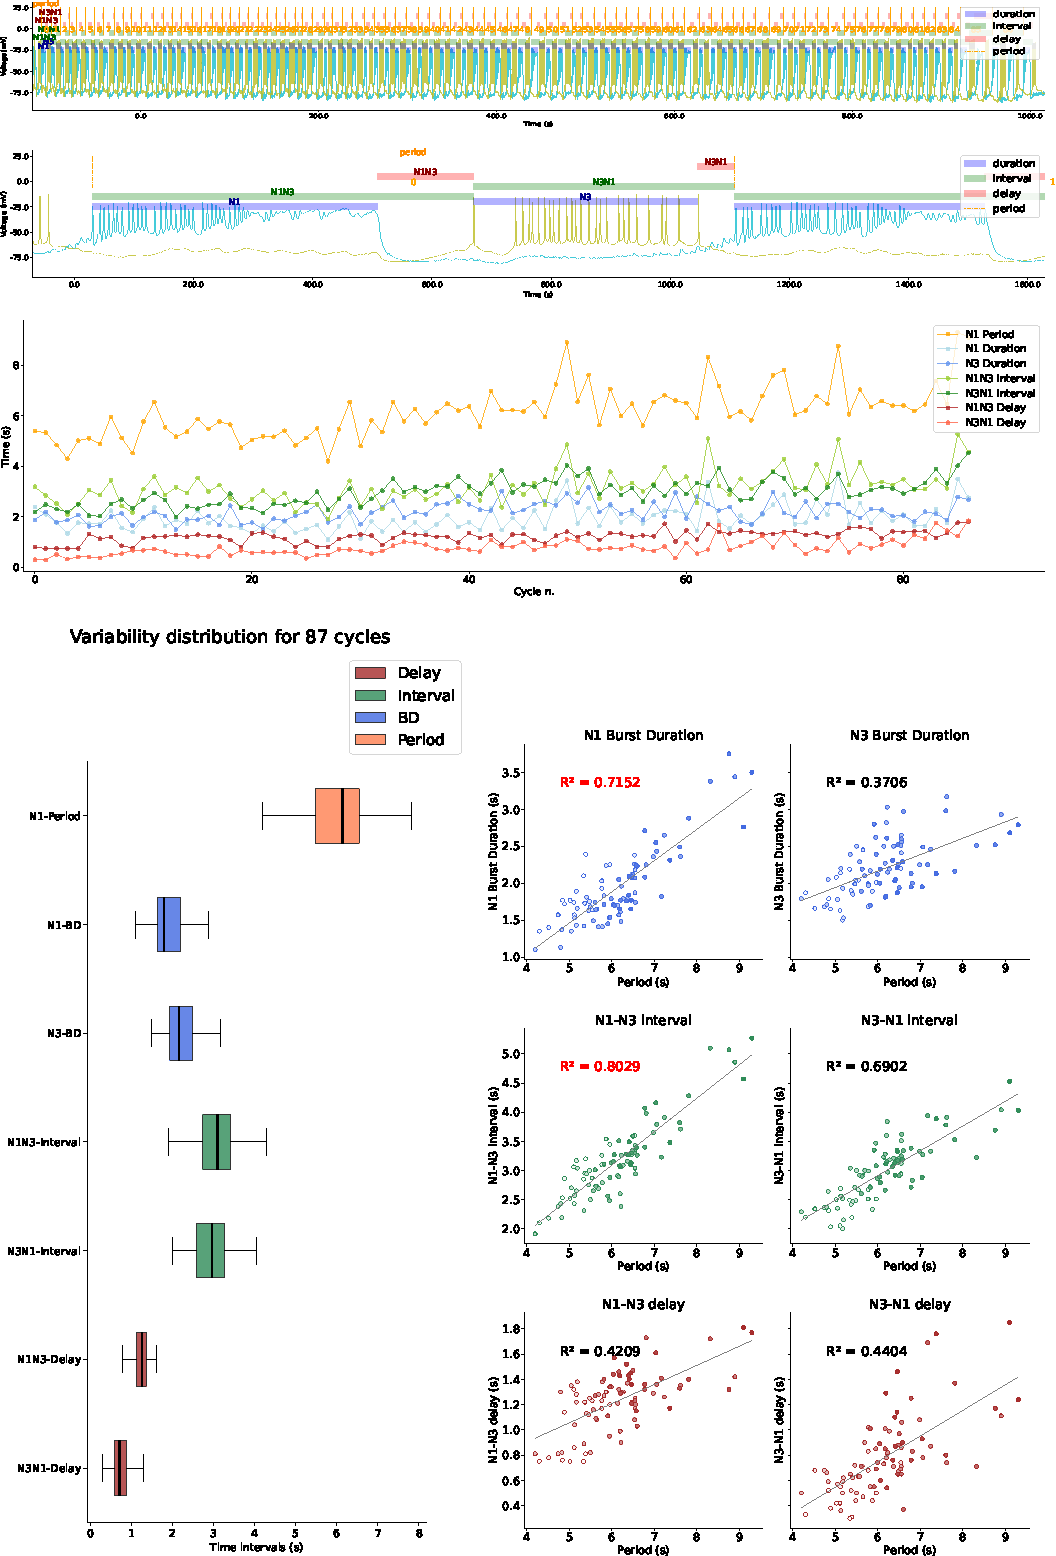
\includegraphics[width=0.9\textwidth]{./img/invariants/data/SUSSEX/prep4_so_driven_2/images/panel_with_intervals.pdf}
	\caption{\textbf{Spontaneous SO neuron modulation restarts}: Panel of interval distributions and dynamical invariants for the two phases in the CPG for spontaneous activity driven by SO neuron. a) Voltage traces for the intracellular recording analyzed for this panel. b) Representation of the time-intervals described. c) Duration of each time interval ($y-axis$) at each cycle. d) Box-plot with the variability distribution of the duration of each time-interval. e) Time-intervals duration against the period for NX-duration (blue), NXNY-Interval (green) and NXNY-Delay (red).}
	\label{fig:so spontaneous invariants 1}
\end{figure}


\begin{figure}[htbp]
	\centering
	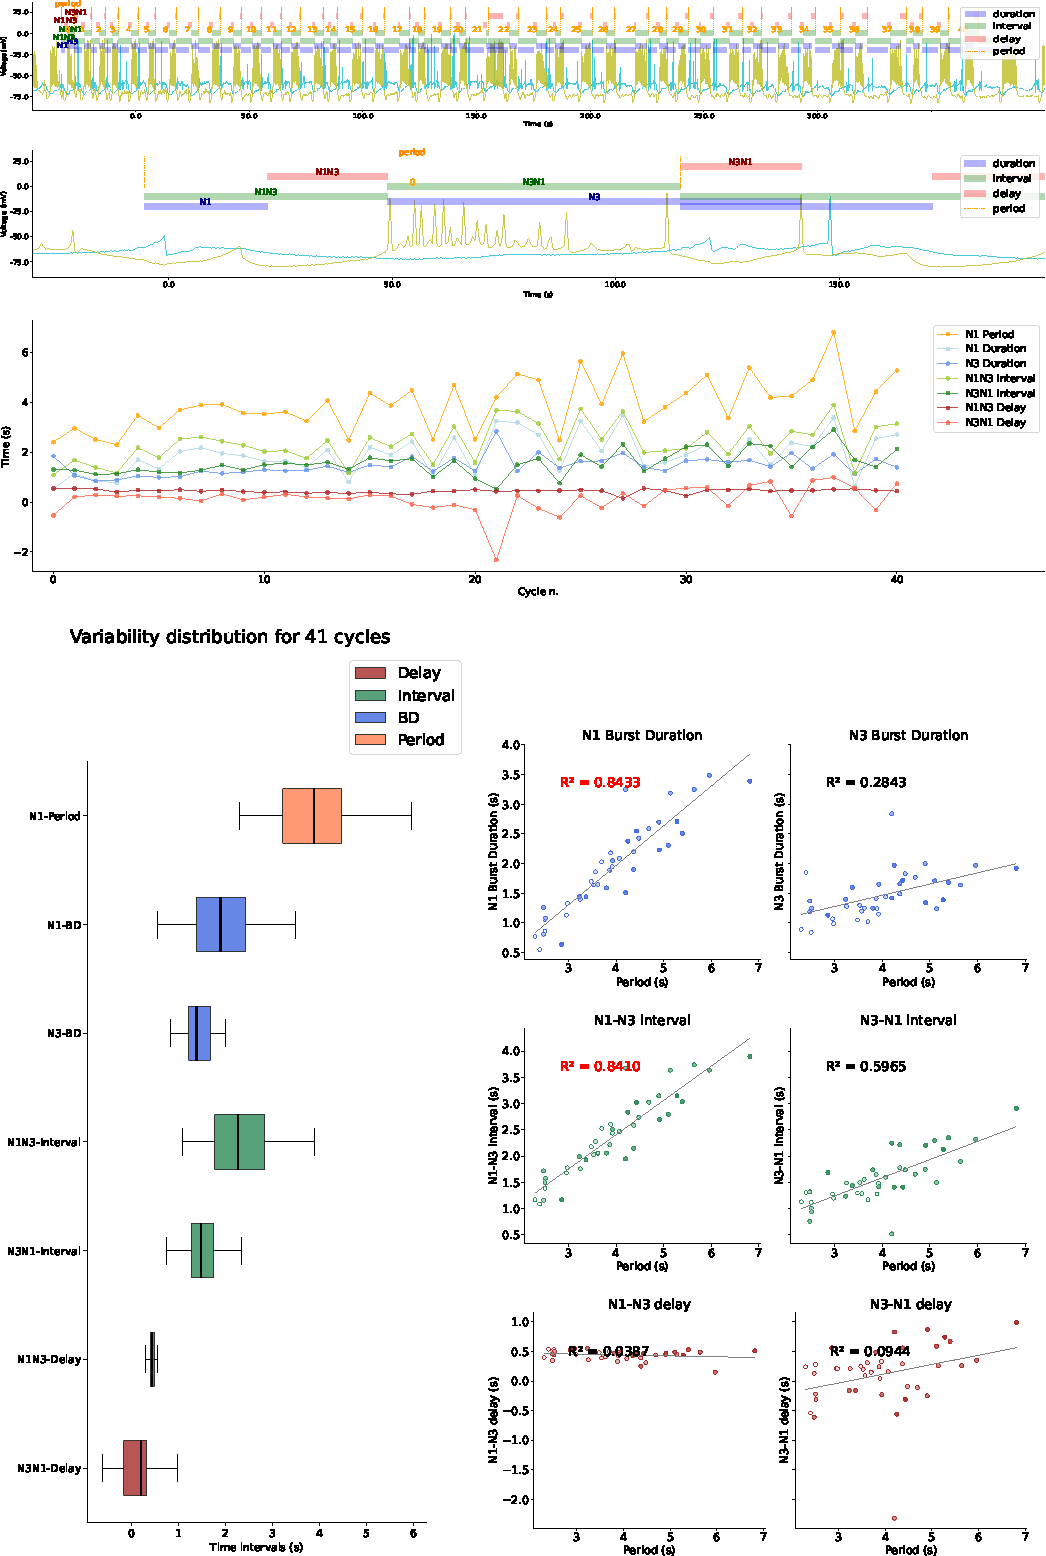
\includegraphics[width=0.9\textwidth]{./img/invariants/data/SUSSEX/SO_driven/images/panel_with_intervals.pdf}
	\caption{\textbf{SO neuron stimulation}: Panel of interval distributions and dynamical invariants for the two phases in the CPG for activity driven by SO neuron induced by its electrical stimulation. a) Voltage traces for the intracellular recording analyzed for this panel. b) Representation of the time-intervals described. c) Duration of each time interval ($y-axis$) at each cycle. d) Box-plot with the variability distribution of the duration of each time-interval. e) Time-intervals duration against the period for NX-duration (blue), NXNY-Interval (green) and NXNY-Delay (red).}
	\label{fig:so induced invariants}
\end{figure}

 
\begin{figure}[htbp]
	\centering
	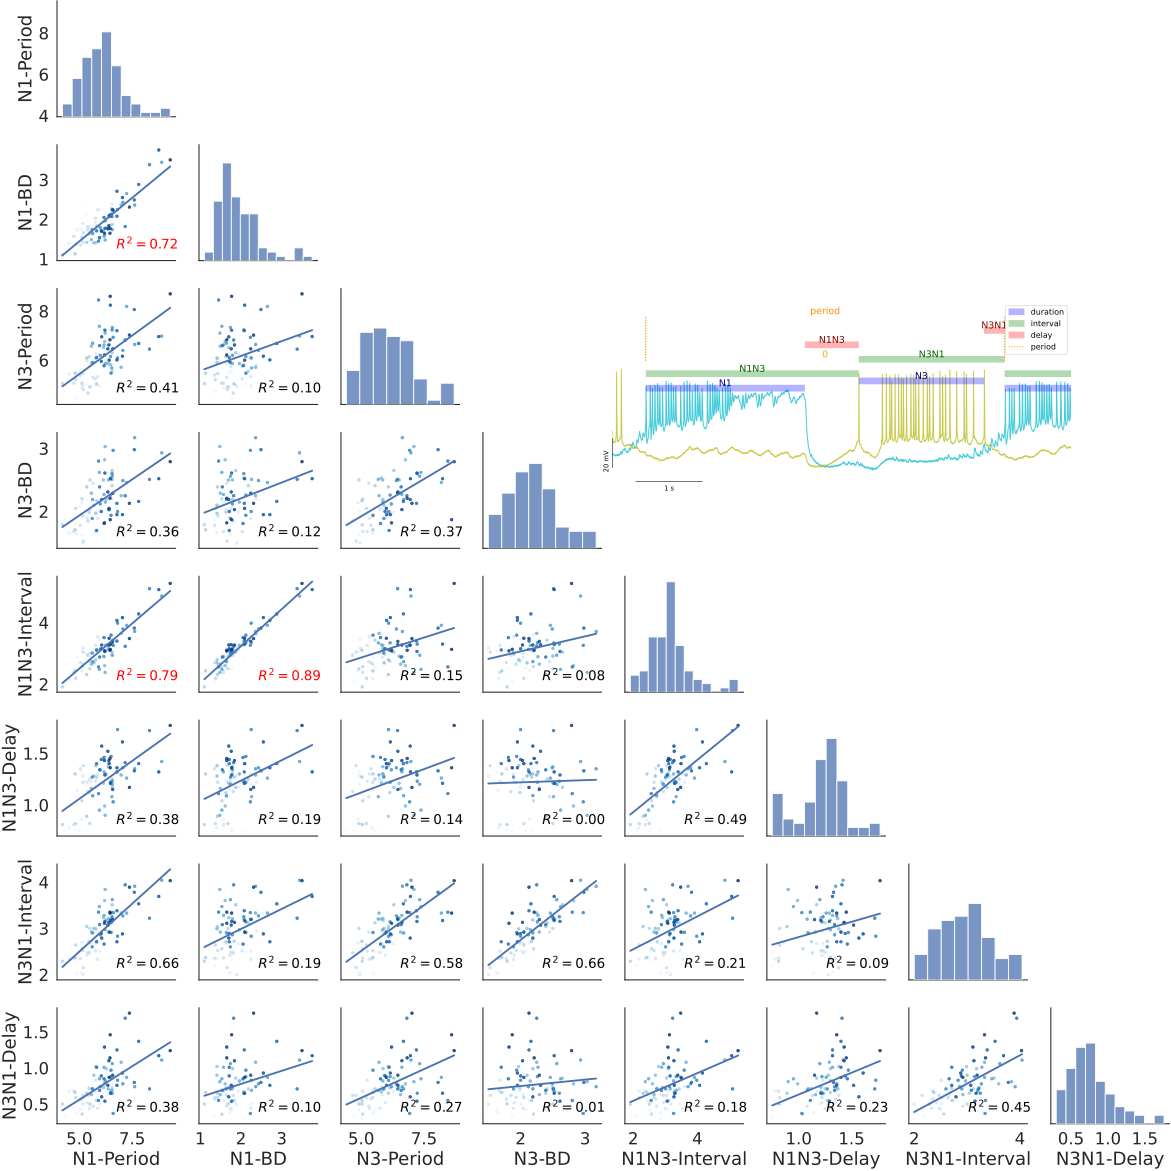
\includegraphics[width=0.48\textwidth]{./img/invariants/data/SUSSEX/prep4_so_driven_2/images/panel_with_pairplot.png}
	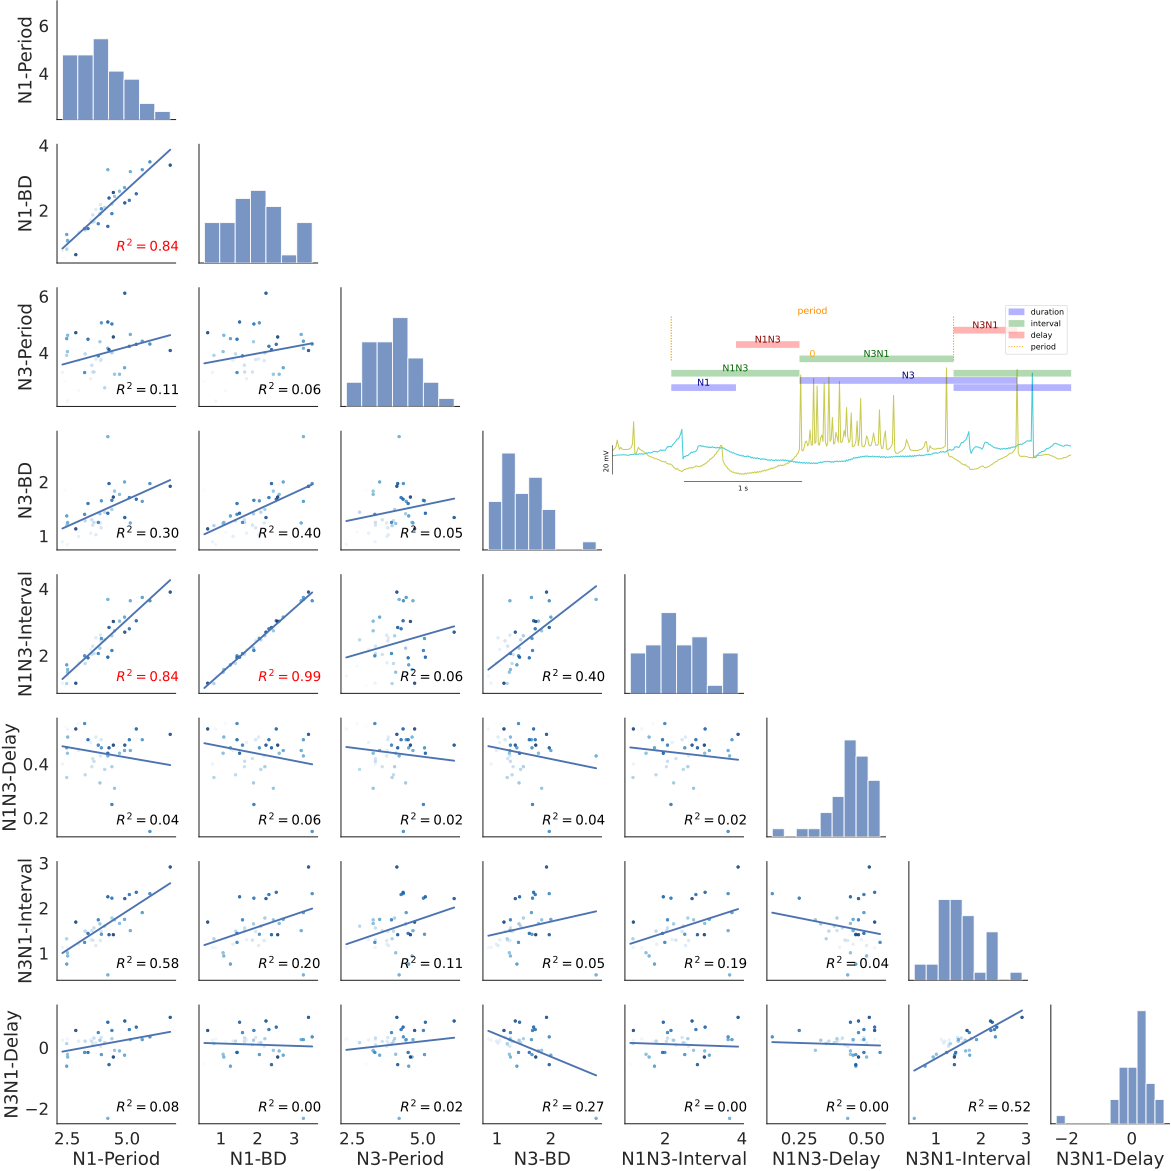
\includegraphics[width=0.48\textwidth]{./img/invariants/data/SUSSEX/SO_driven/images/panel_with_pairplot.png}
	\caption{Panel of the pairplots for all possible combinations between the time intervals for two phases in the CPG recordings for (left) spontaneous SO rhythm modulation and (right) the induced SO rhythm modulation.}
	\label{fig:so pairplot comparison}
\end{figure}

\newpage
\subsection{Invariants in MLN stimulation driven activity}
The snail's lips are connected to the cerebral ganglia by the MLN (median lip nerves). It is possible to activate CPG activity by its stimulation, simulating the initiation of the rhythm in food presence \parencite{staras_electrophysiological_1999}. This nerve directly stimulates the N1M interneuron, in charge of the initiation of the rhythm, associated to the protraction phase. In Fig. \ref{fig:mln stimulation} the variability and time-intervals correlations are characterized for a recording of this induced stimulation. We can see in that figure that there is a strong linear correlation in the panel, leading the rhythm completely by N1 phase. This is visible in the robust dynamical invariant between N1 burst duration and the period and by N1N3 interval and the period. It is also important that no other intervals have relation with the period, so both N2 and N3 phases remain constant. Note that the N1 burst duration takes a wide range of values for its duration, even at really low ranges, shorter than N3 burst for example. This is also clearly represented in the figure in the third row, where N1 burst duration and N1N3 interval robustly follow the period. 
In Fig. \ref{fig:mln stimulation pairplot} all possible combination of time-intervals for two phases are represented. We can see there other strongly related intervals: N1N3 interval with N1 burst duration, which again highlights the steadiness of N2 phase. 
These results suggest that during the MLN stimulation, the feeding rhythm variability is lead by N1 phase, activating the rhythm and stabilizing the activity. 
%Also there are some other intervals that present a tendency to a linear relation with $R^2$ close to 0.7: N3N1 Interval and N3 burst duration, and N1N3 delay and N1N3 interval 


\begin{figure}[htbp]
	\centering
	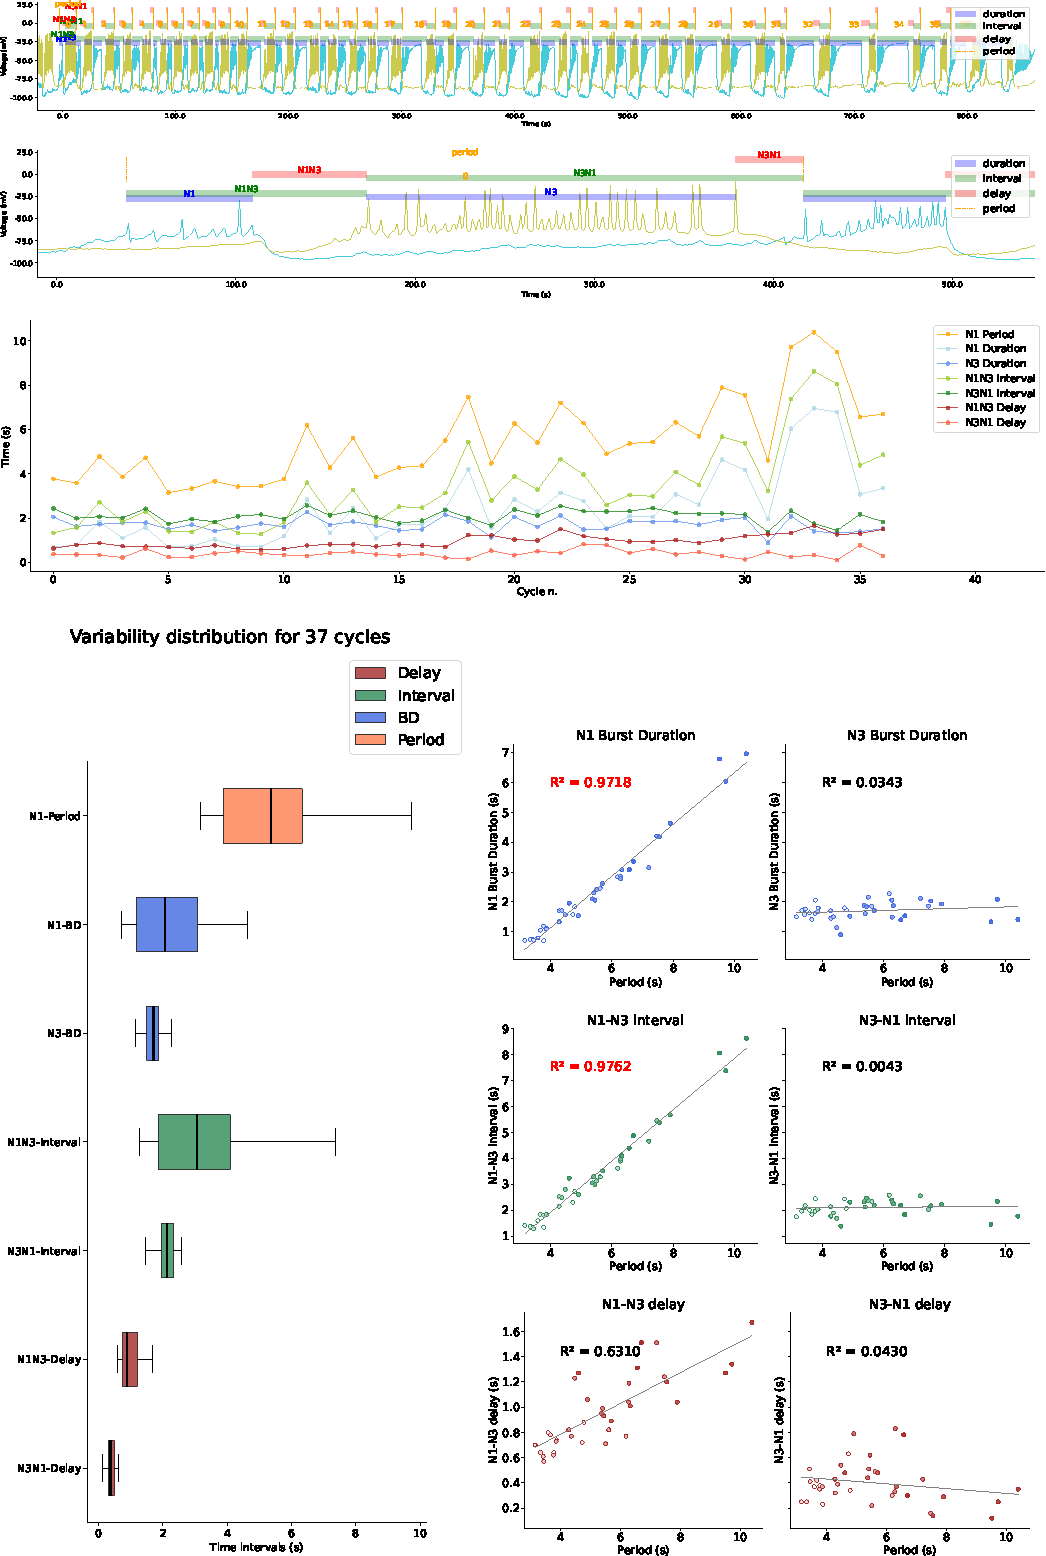
\includegraphics[width=0.9\textwidth]{./img/invariants/data/SUSSEX/MLN_driven/images/panel_with_intervals.pdf}
	\caption{\textbf{MLN stimulation}: Panel of interval distributions and dynamical invariants for the three phases in the CPG under MLN Medium Lip Nerve (MLN) stimulation. a) Voltage traces for the intracellular recording analyzed for this panel. b) Representation of the time-intervals described. c) Duration of each time interval ($y-axis$) at each cycle. d) Box-plot with the variability distribution of the duration of each time-interval. e) Time-intervals duration against the period for NX-duration (blue), NXNY-Interval (green) and NXNY-Delay (red).}
	\label{fig:mln stimulation}
\end{figure}


\begin{figure}[htbp]
	\centering
	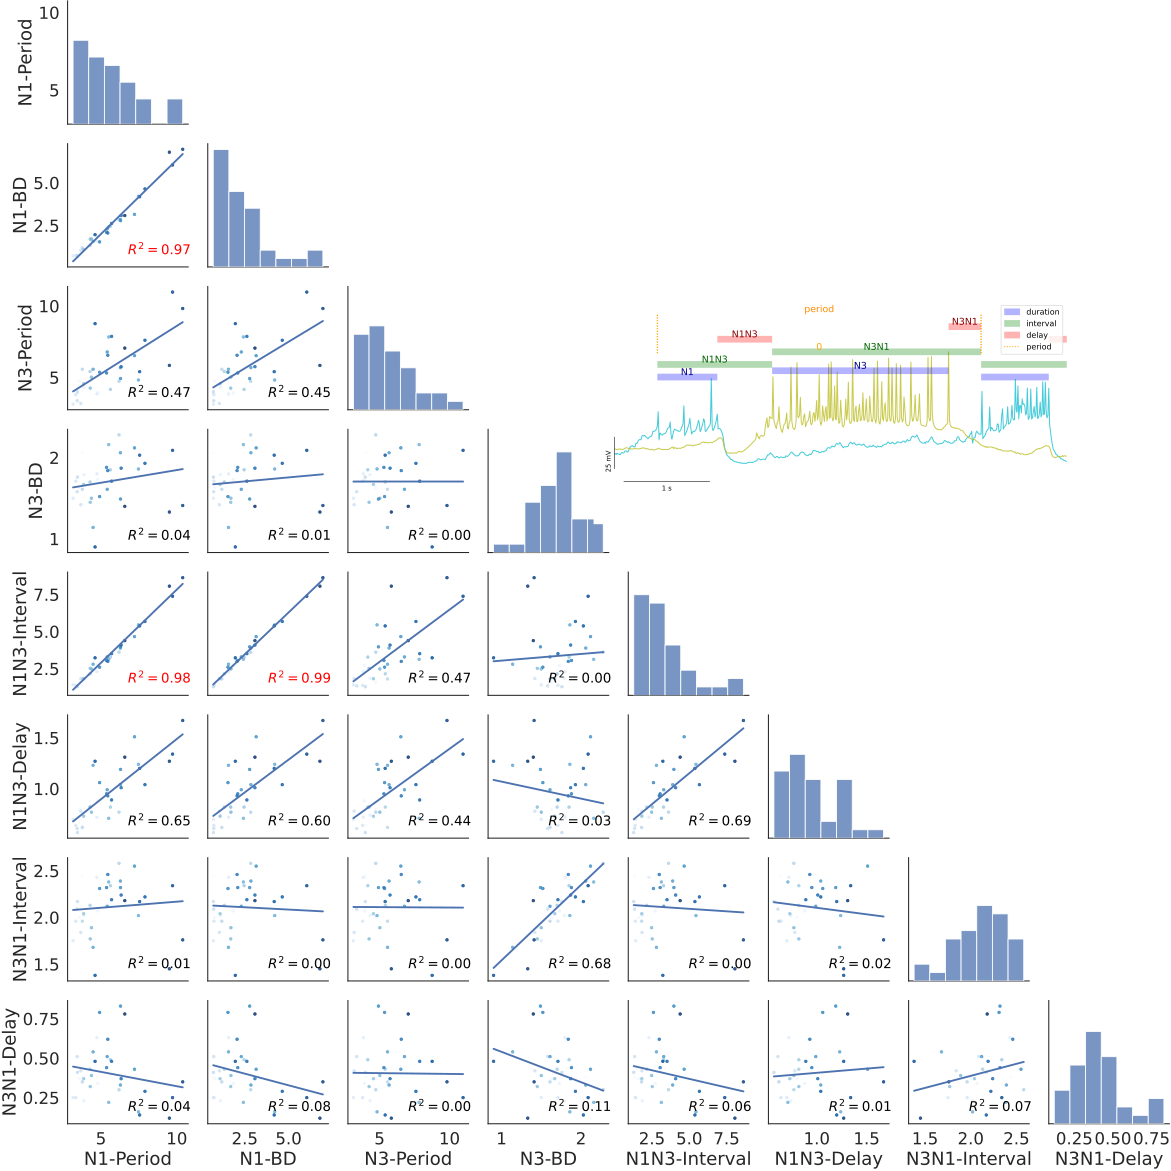
\includegraphics[width=0.9\textwidth]{./img/invariants/data/SUSSEX/MLN_driven/images/panel_with_pairplot.png}
	\caption{\textbf{MLN stimulation}:Pairplot with all possible combinations in the intervals.}
	\label{fig:mln stimulation pairplot}
\end{figure}

\newpage
\subsection{Invariants in CVa1 driven activity induced by electrical stimulation}
CV1a neuron is part of a larger population of CBIs that is influeced by sucrose, which can drive the rhythmic activity in that group of neurons. CBIs are connected by mutual excitation to interneuron N1M, involved in the rhythm initation (see Fig. \ref{fig:feeding distribution}). Therefore, it can be expected to observe in this case a stronger role of N1 phase in the variability distribution. For this case, there are four examples of different recordings, represented in figures \ref{fig:cv1a 1 2phases} to \ref{fig:cv1a 3 2phases}. In the first three panels, we can see that the stronger relation is in N1 burst duration, specially in the first case where there is a strong sequential dynamical invariant with $R^2>0.9$. The rest of the intervals conforming that sequence were not strongly related, being N3 phase more variable than the N2 phase, barely presenting variability and with no linear correlation with the period. It is interesting to highlight that not in all cases where the variability was larger, the correlation to the period was also larger, as it is the case in example 3 in Figs. \ref{fig:cv1a 2 2phases} and \ref{fig:cv1a 4 2phases}. In those examples, the variability in N3 neuron is large but it is not related to the period. Seeing the third figure in each of those panels, we can explain it by the opposite direction of the changes in N3 (dark blue),  N1 (light blue) and the period (orange), pointing that the N3 burst is adapting to the N1 strongest variability. This distribution is maintained for the three first cases, however, in the last case this is shifted. In the example characterized in Fig. \ref{fig:cv1a 3 2phases}, the N3 burst duration has a stronger linear relation with the period than N1, presenting also a larger variability. During that period the electrode stimulating CV1a slipped away and the stimulation was not as effective as it was in the rest of the examples. We can appreciate in the correlation between N1 and the period that there are some points white-colored that correspond to the beginning of the trace, which might look as outliers but present a tendency to a linear regression.  Although this was not a methodic study, we decided to include this case since it represents the sensitivity of the circuit to changes in the context, redistributing the activity between the different phases in a flexible way, in this case from N1 to N3.

Finally, Fig. \ref{fig:cv1a pairplot comparison} depicts the plots for two phases for each panel. In one of the recordings, the N2 phase could be well identified, and the corresponding pairplot for three phases is in the Appendix \ref{fig:cv1a 4 3phases pairplot}. In the pairplot, again we see a similar distribution in all figures except of the last one, where there are new correlations, present in the N3 burst duration with the N3N1 interval. Also there is a correlation of a negative slope in the first case, in case N3-BD and N3N1 delay, representing a regular overlapping of N1 and N3 phases. 
%
%%and the complete map of their locations is shown in Figure 3A. https://static-content.springer.com/esm/art%3A10.1186%2F2042-1001-2-4/MediaObjects/13232_2011_20_MOESM3_ESM.jpeg
%Sucrose drives rhythmic activity in CBIs activating the feeding circuit by the conection
%\paragraph{Example 1}

\begin{figure}[htbp]
	\centering
	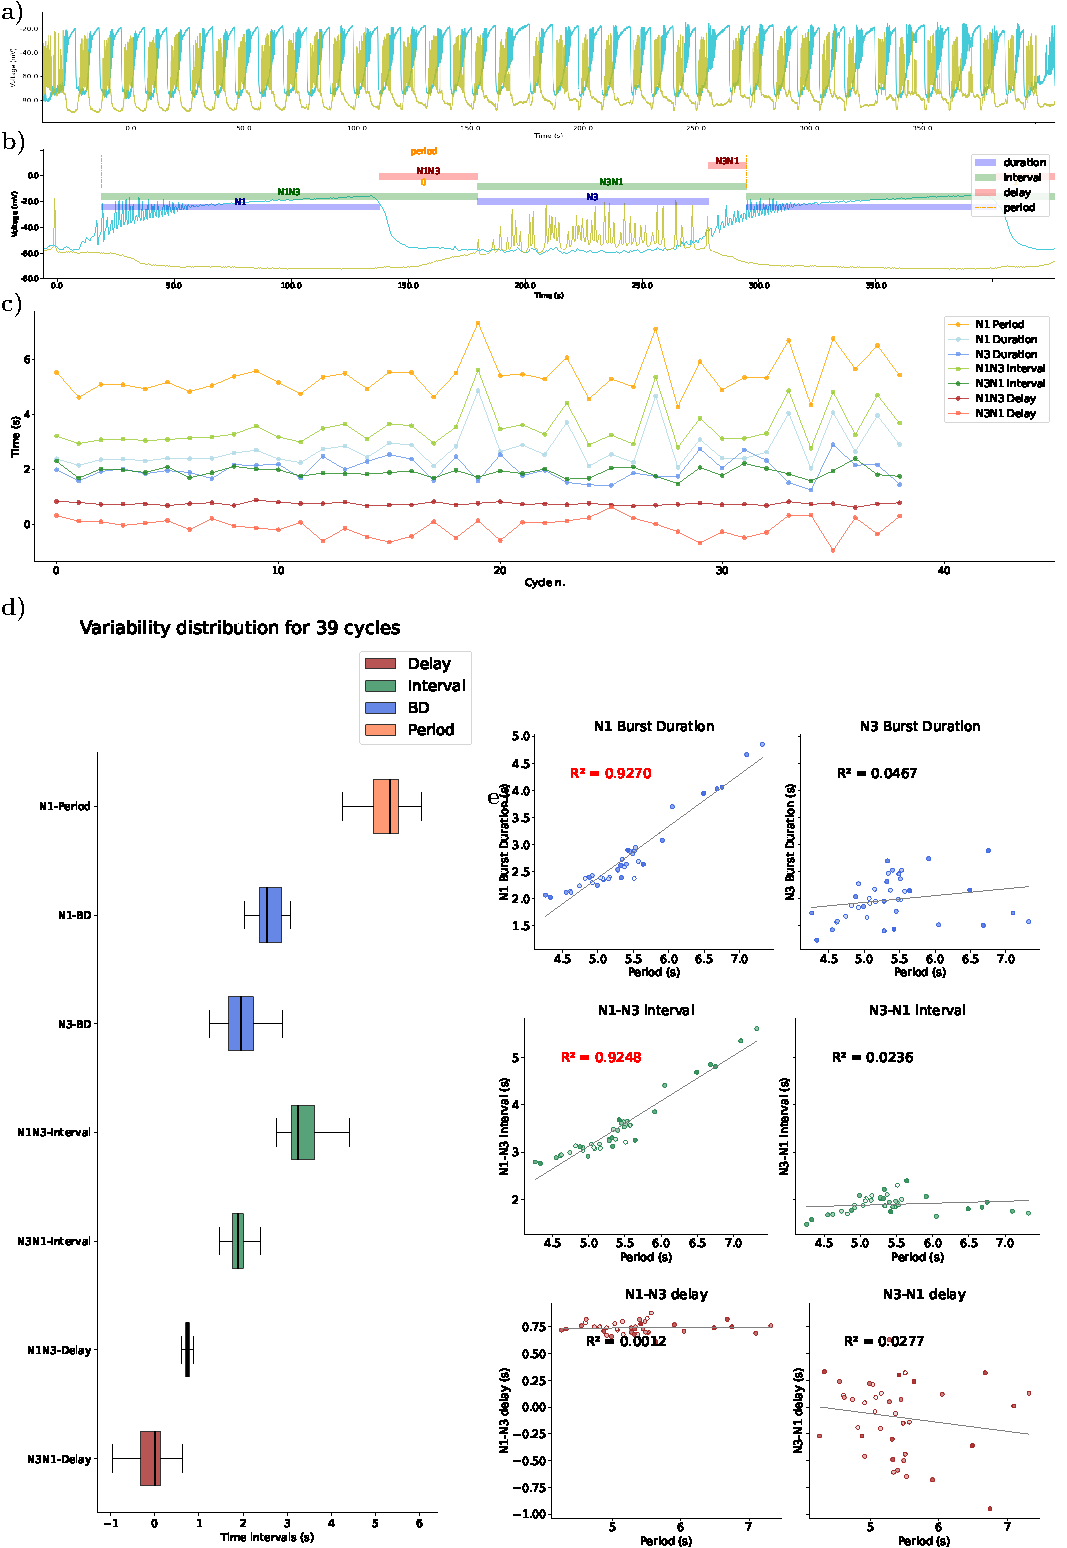
\includegraphics[width=0.9\textwidth]{./img/invariants/data/SUSSEX/CV1a_driven1/images/2phases/panel_with_intervals.pdf}
	\caption{\textbf{CV1a driven case 1}: Panel of interval distributions and dynamical invariants for the two phases in the CPG under CV1a stimulation. a) Voltage traces for the intracellular recording analyzed for this panel. b) Representation of the time-intervals described. c) Duration of each time interval ($y-axis$) at each cycle. d) Box-plot with the variability distribution of the duration of each time-interval. e) Time-intervals duration against the period for NX-duration (blue), NXNY-Interval (green) and NXNY-Delay (red).}
	\label{fig:cv1a 1 2phases}
\end{figure}

%\paragraph{Example 2}


\begin{figure}[htbp]
	\centering
	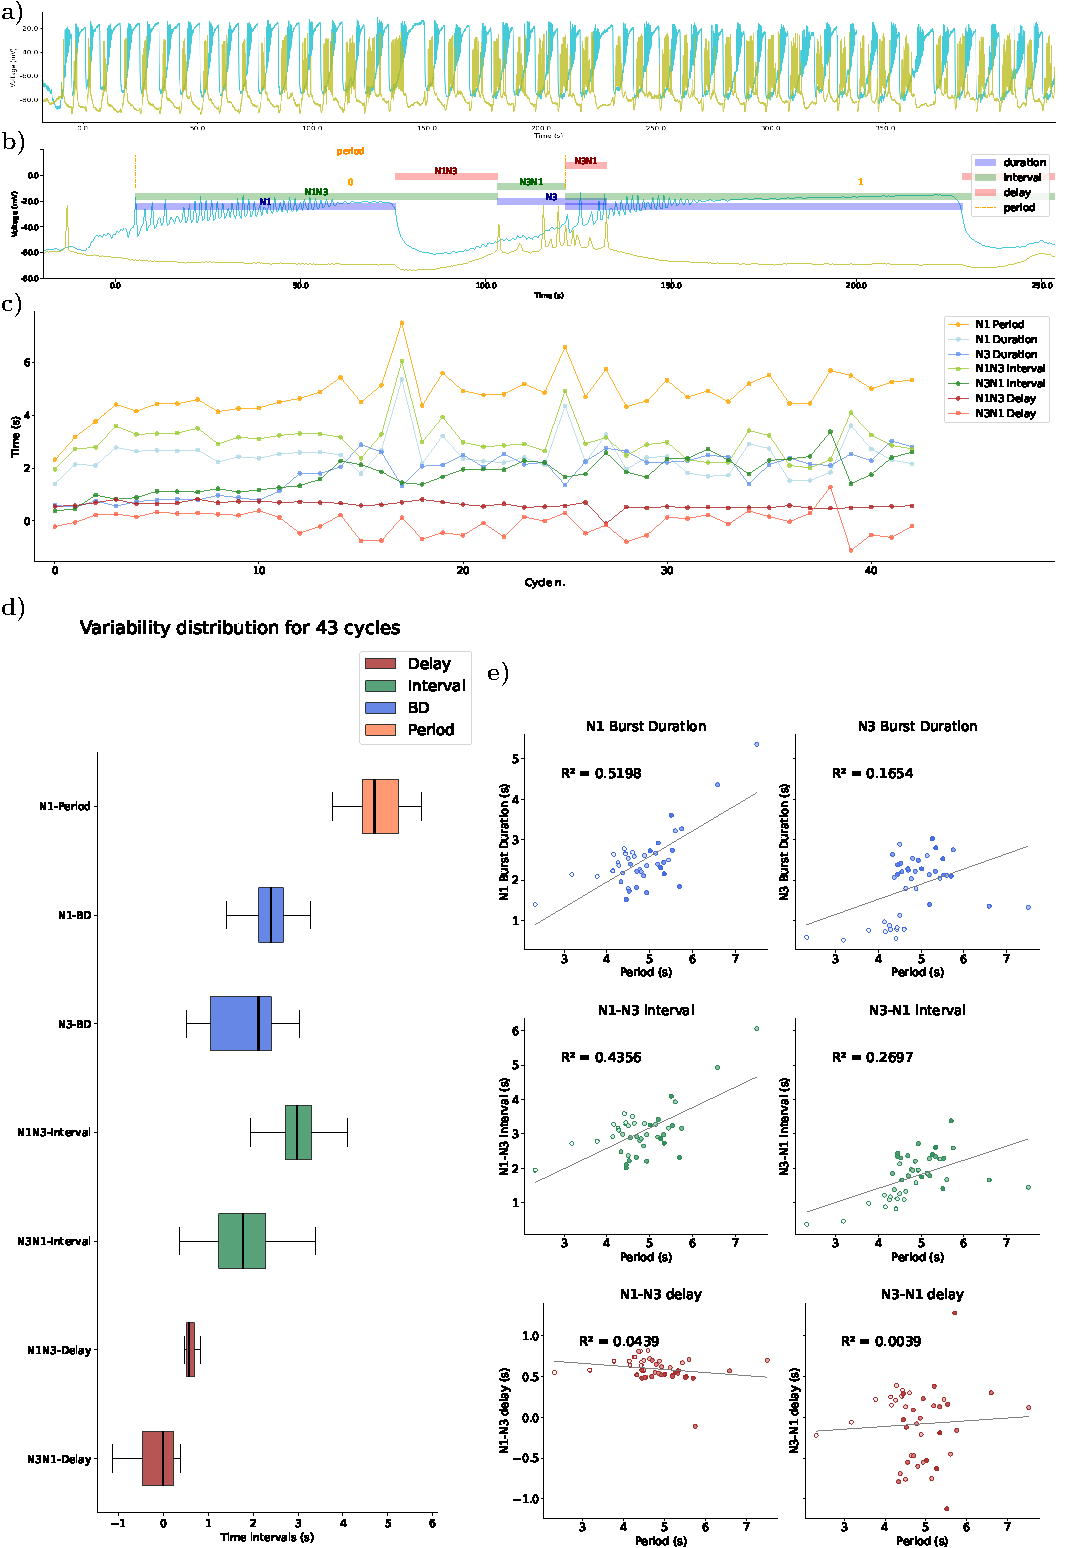
\includegraphics[width=0.9\textwidth]{./img/invariants/data/SUSSEX/CV1a_driven2/images/panel_with_intervals.pdf}
	\caption{\textbf{CV1a driven case 2}: Panel of interval distributions and dynamical invariants for the two phases in the CPG under CV1a stimulation. a) Voltage traces for the intracellular recording analyzed for this panel. b) Representation of the time-intervals described. c) Duration of each time interval ($y-axis$) at each cycle. d) Box-plot with the variability distribution of the duration of each time-interval. e) Time-intervals duration against the period for NX-duration (blue), NXNY-Interval (green) and NXNY-Delay (red).}
	\label{fig:cv1a 2 2phases}
\end{figure}


%\paragraph{Example 4}

\begin{figure}[htbp]
	\centering
	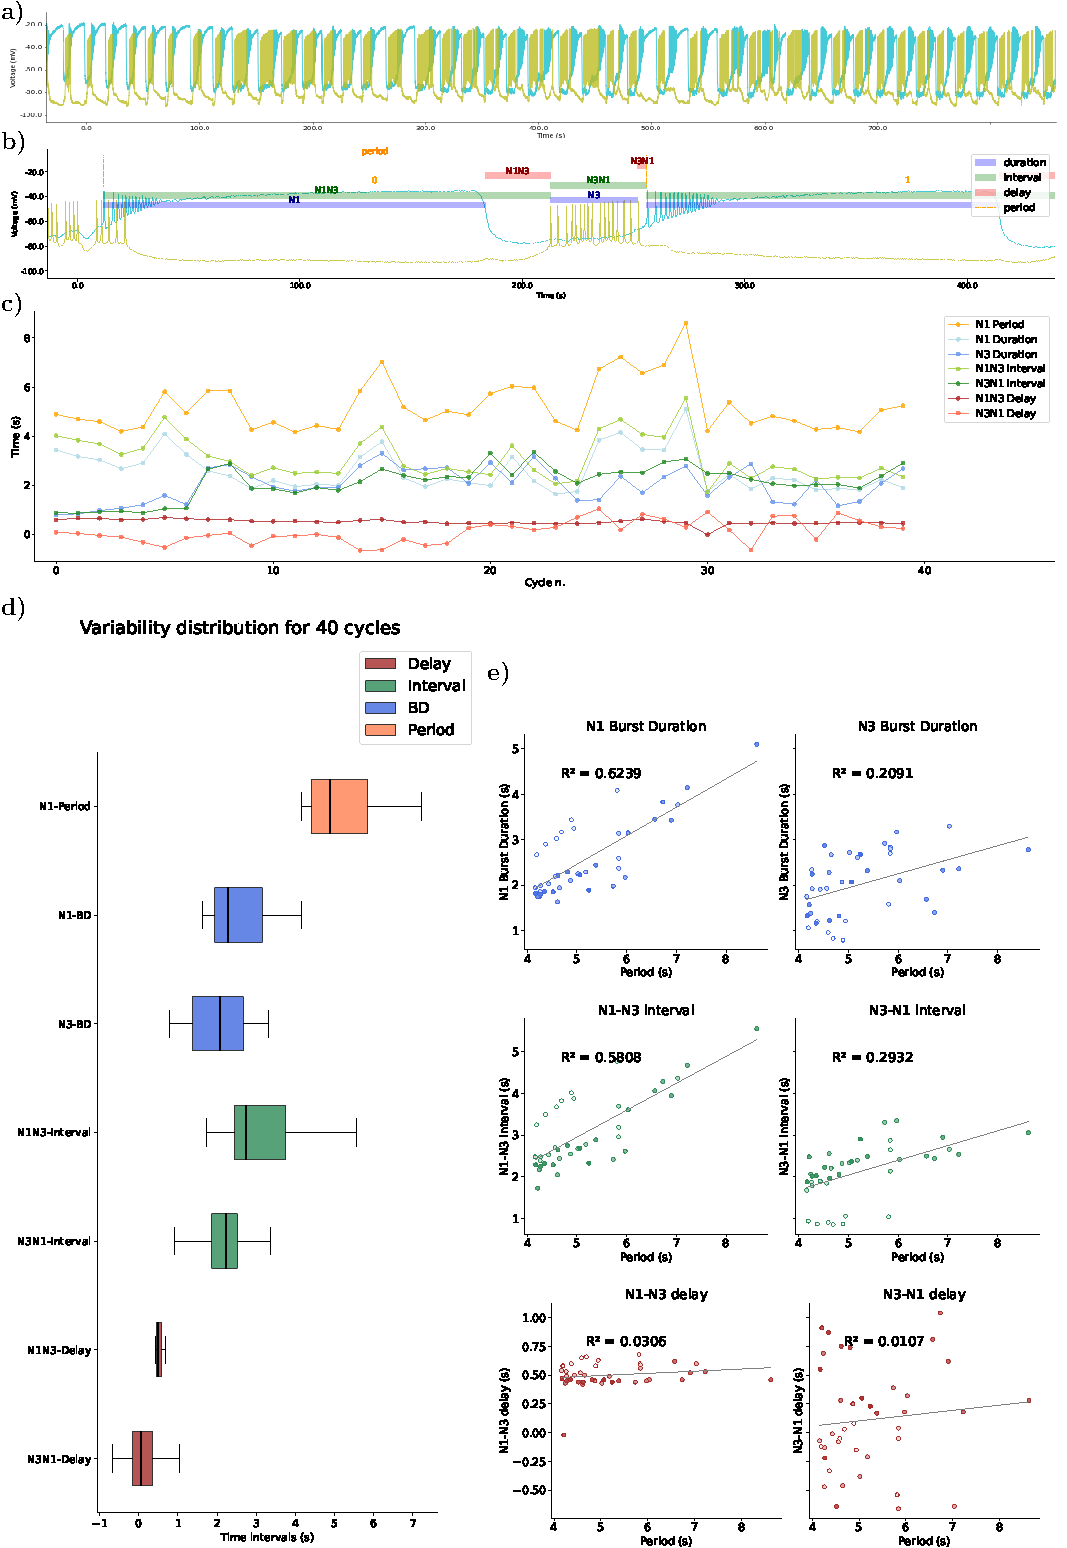
\includegraphics[width=0.9\textwidth]{./img/invariants/data/SUSSEX/CV1a_driven4/images/2phases/panel_with_intervals.pdf}
	\caption{\textbf{CV1a driven case 3}: Panel of interval distributions and dynamical invariants for the two phases in the CPG under CV1a stimulation. a) Voltage traces for the intracellular recording analyzed for this panel. b) Representation of the time-intervals described. c) Duration of each time interval ($y-axis$) at each cycle. d) Box-plot with the variability distribution of the duration of each time-interval. e) Time-intervals duration against the period for NX-duration (blue), NXNY-Interval (green) and NXNY-Delay (red).}
	\label{fig:cv1a 4 2phases}
\end{figure}


%\paragraph{Example 3}


\begin{figure}[htbp]
	\centering
	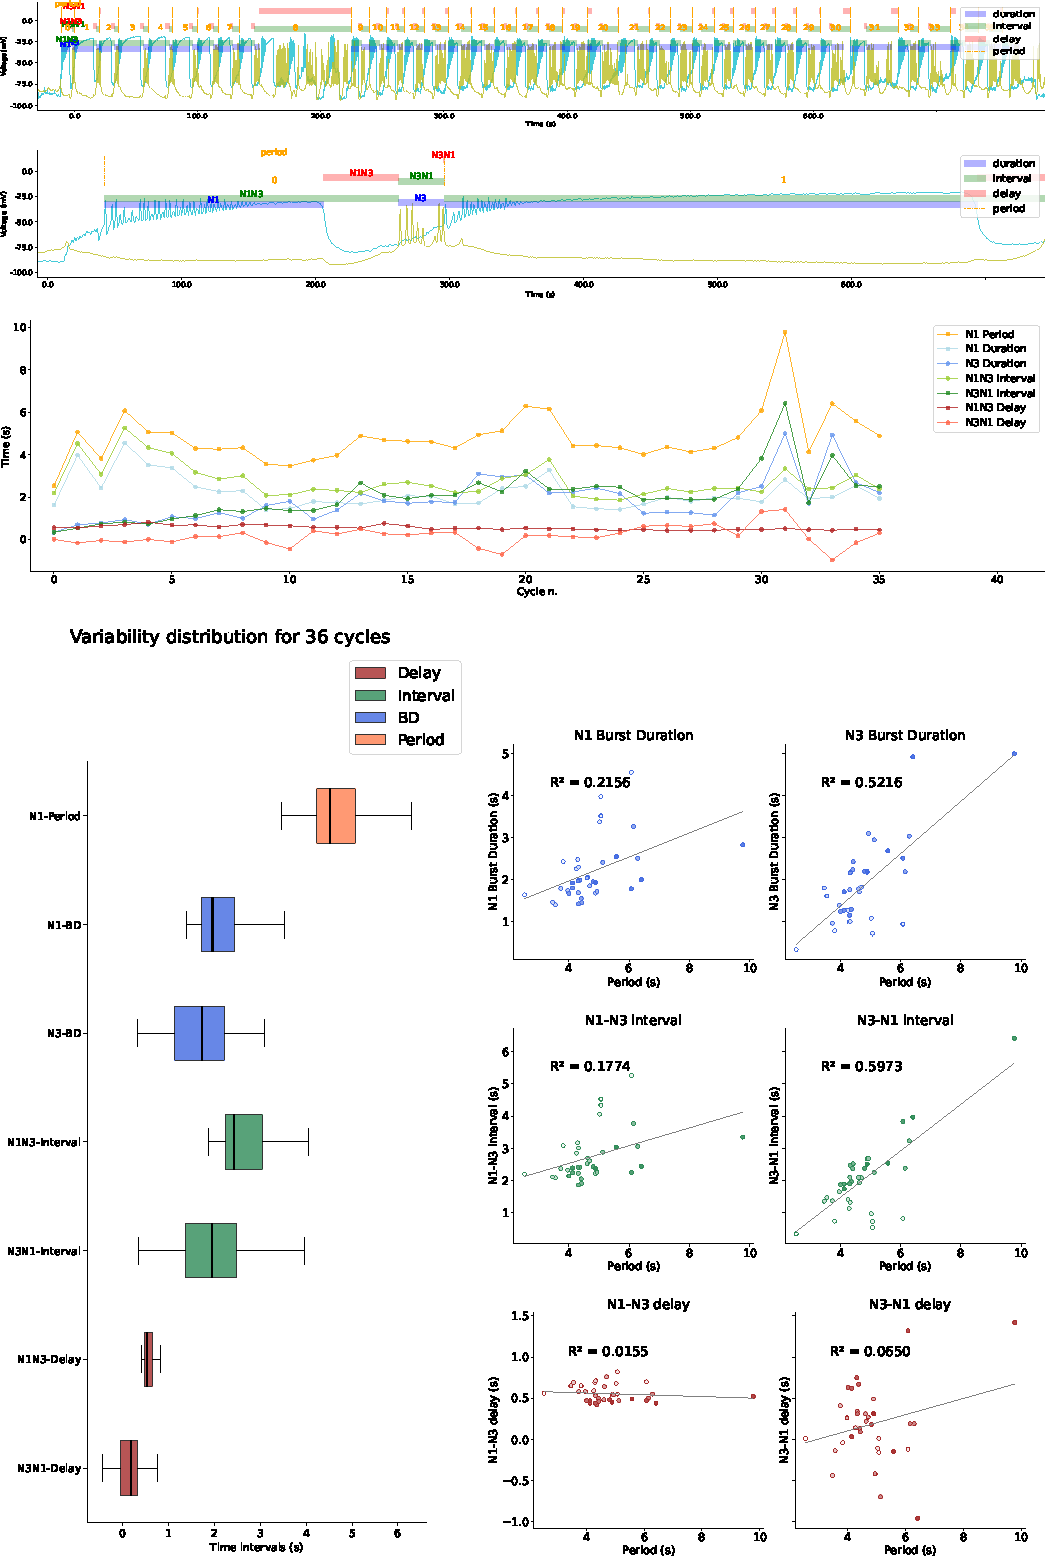
\includegraphics[width=0.9\textwidth]{./img/invariants/data/SUSSEX/CV1a_driven3/images/panel_with_intervals.pdf}
	\caption{\textbf{CV1a driven case 4}: Panel of interval distributions and dynamical invariants for the two phases in the CPG under CV1a stimulation. a) Voltage traces for the intracellular recording analyzed for this panel. b) Representation of the time-intervals described. c) Duration of each time interval ($y-axis$) at each cycle. d) Box-plot with the variability distribution of the duration of each time-interval. e) Time-intervals duration against the period for NX-duration (blue), NXNY-Interval (green) and NXNY-Delay (red).}
	\label{fig:cv1a 3 2phases}
\end{figure}




\begin{figure}[htbp]
	\centering
	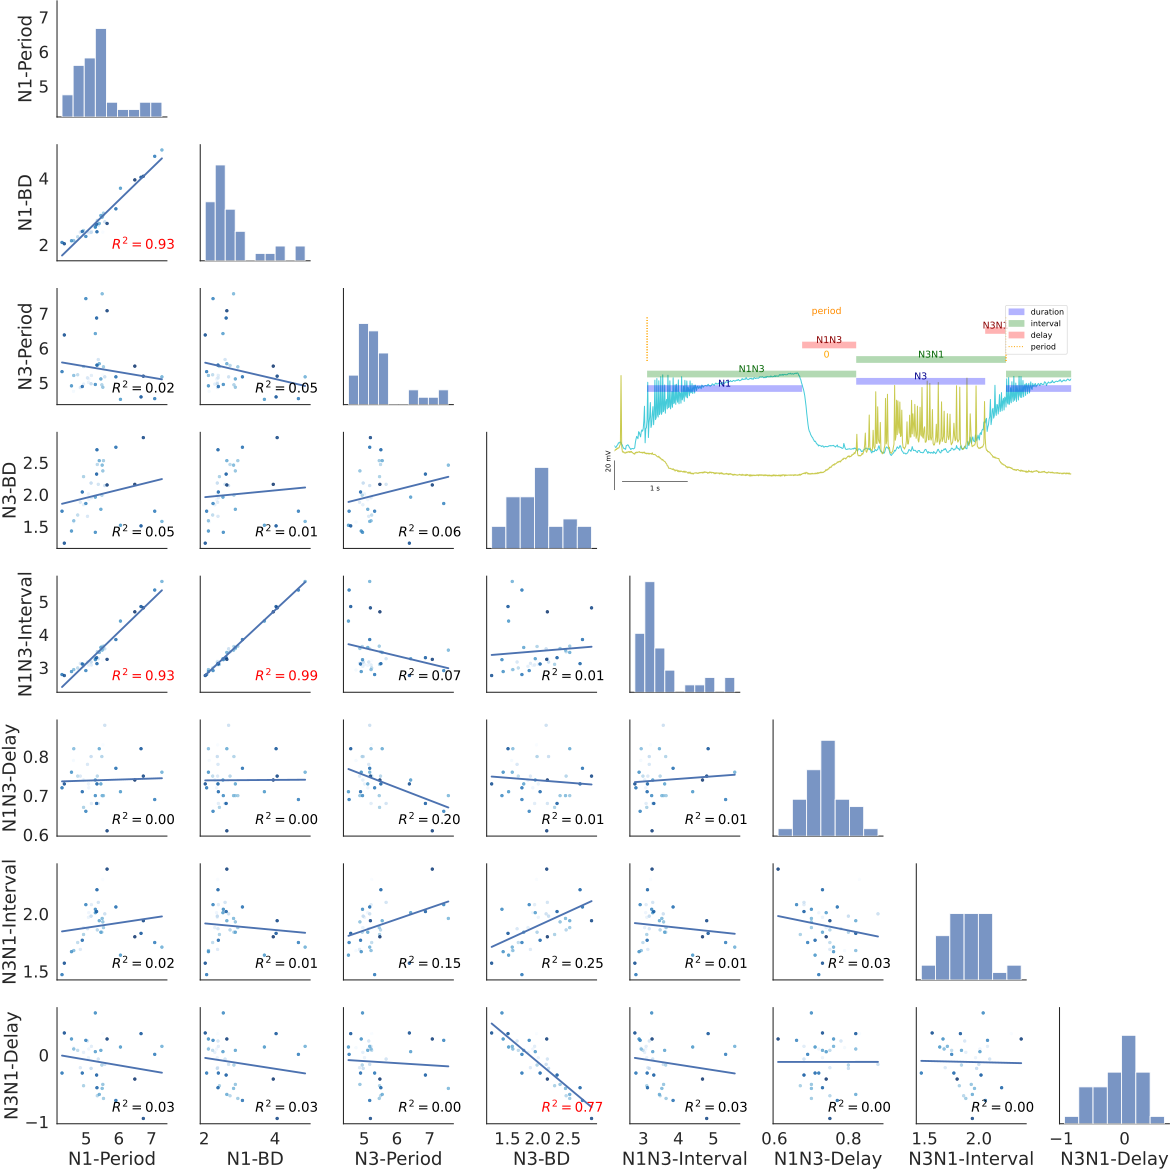
\includegraphics[width=0.48\textwidth]{./img/invariants/data/SUSSEX/CV1a_driven1/images/2phases/panel_with_pairplot.png}
	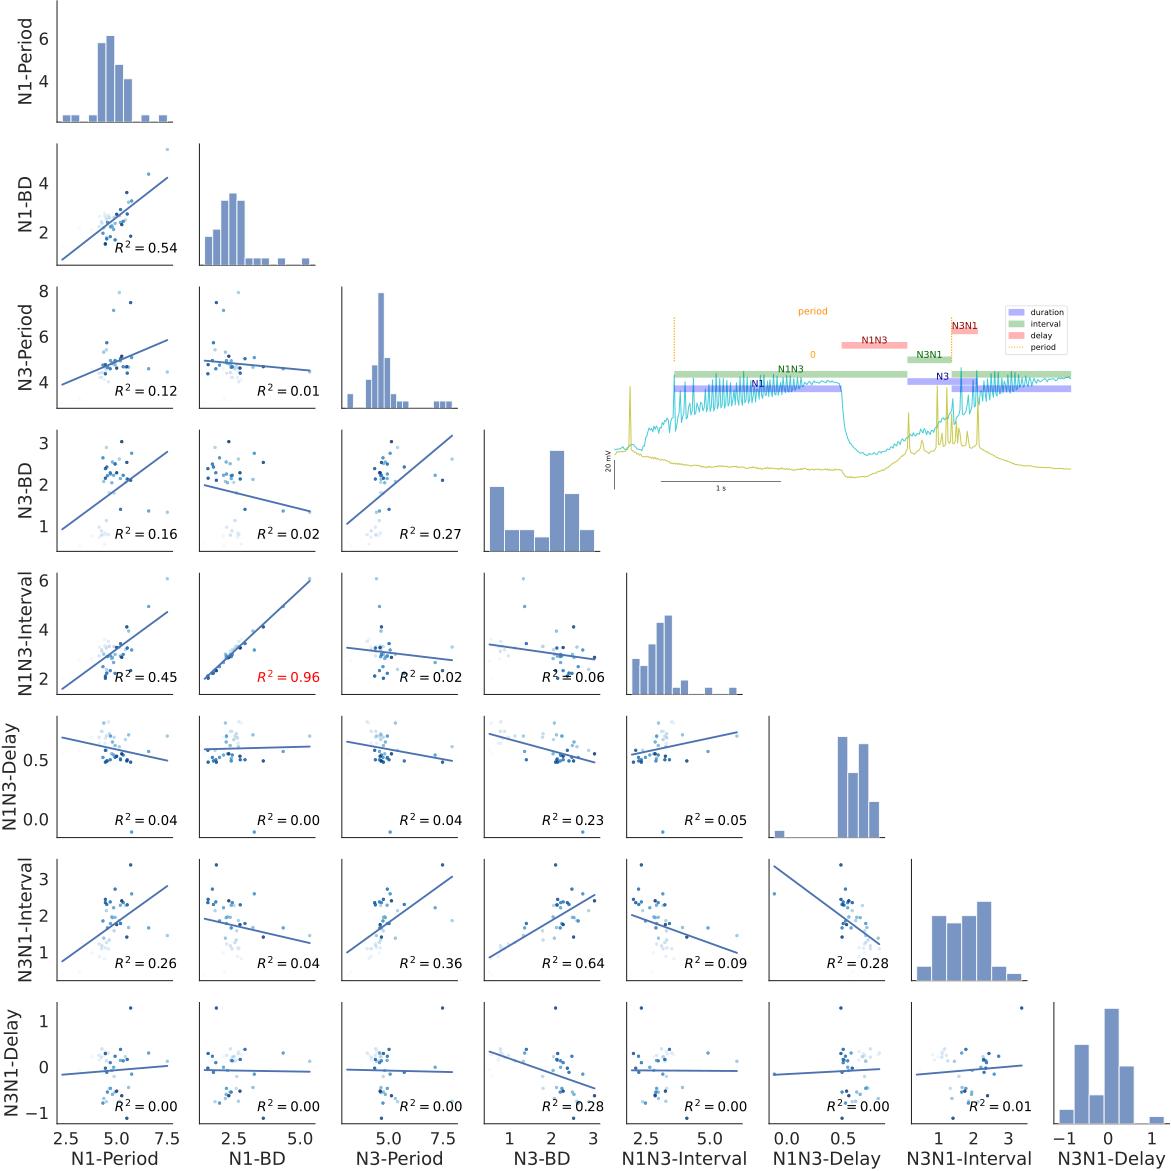
\includegraphics[width=0.48\textwidth]{./img/invariants/data/SUSSEX/CV1a_driven2/images/panel_with_pairplot.png}
	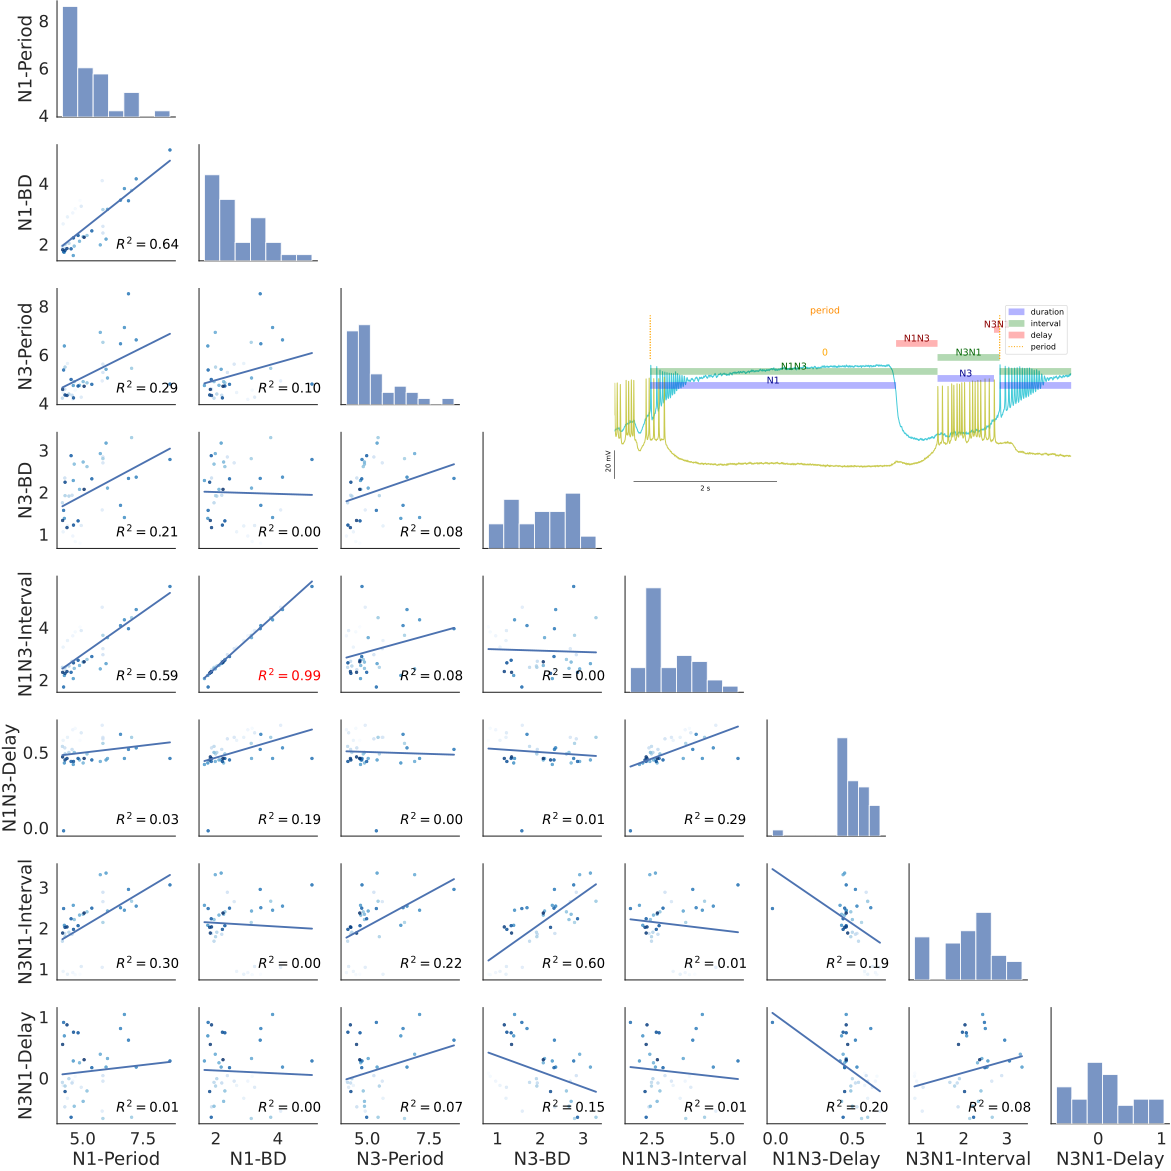
\includegraphics[width=0.48\textwidth]{./img/invariants/data/SUSSEX/CV1a_driven4/images/2phases/panel_with_pairplot.png}
	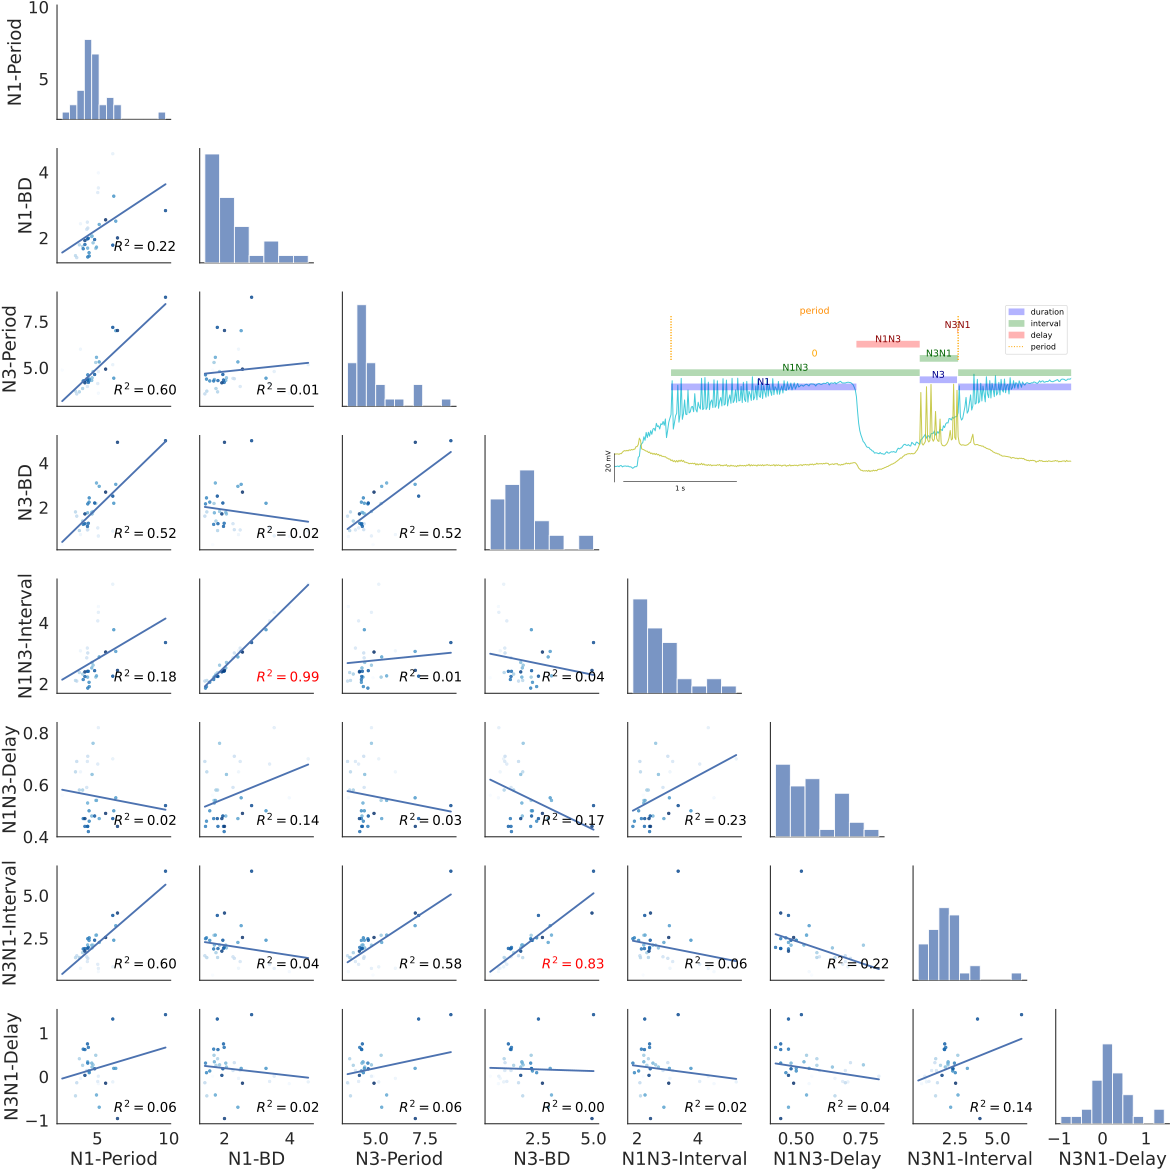
\includegraphics[width=0.48\textwidth]{./img/invariants/data/SUSSEX/CV1a_driven3/images/panel_with_pairplot.png}
	\caption{Panel of the pairplots for all possible combinations between the time intervals for two phases (N1 and N3) in the CPG recordings for the four examples of induced CV1a neuron modulation recordings.}
	\label{fig:cv1a pairplot comparison}
\end{figure}

\subsection{Summary of changes in the invariants due to stimulation}
Figure \ref{fig:results summary} shows the time-interval relationships for four examples in each stimulation case studied in this section. We can see that the relations between the intervals change as the source of the stimulation changes (including the case of spontaneous activity).

In the case of the spontaneous activity, there is a dynamical invariant in the N3 phase intervals, e.g., see the strong correlation between N3 burst duration and the period; while there is no relation between N1 burst duration and the period. When the stimulation is induced by SO, we can see a change in the distribution of the variability, being N1 burst duration and N1N3 interval the strongest ones related to the period, but N3 phase presenting also some tendency to a linear relation visible in the relation of N3 burst duration with specific intervals as the period, N1N3 interval and N3N1 interval. When stimulating MLN and CV1a, the strongest correlation was in N1 with no relation of N3 phase to the period (in contrast to the SO-driven results). MLN case showed a clear and strong linear relation to the period in a large range of values of the duration of the time-intervals, i.e., for low values of the intervals duration there were also low values for the period duration. 

Each of these cases represent a different source of modulation or initiation in the rhythm. The spontaneous case might be during a hunger phase with no food, with longer phases of N3 activation but constant intervals for N1 (protraction) and N2 (rasp) phases. SO modulation is associated to sucrose stimulus, changing the importance of each phase, enhancing the protraction, as it is the case of MLN, when the stimulus of the lip might prioritize an effective protraction activity. Also, the CV1a modulatory neuron used for the rhythm activation presented a distribution between the protraction (N1) and swallow (N3) phases. This redistribution indicated by the changes in the sequential dynamical invariants points to the relation of the variability and the functional context of the feeding motor activity.

\begin{figure}[htbp]
\centering
\begin{minipage}{\textwidth}
	\begin{minipage}{0.49\textwidth}
		\centering
		\begin{overpic}[width=\textwidth]{img/invariants/data/SUSSEX/Summary/output_pairplot_spon.pdf} % Base image
		\put(50,55){ % Position the second image (70%, 60% of width/height of figure1)
			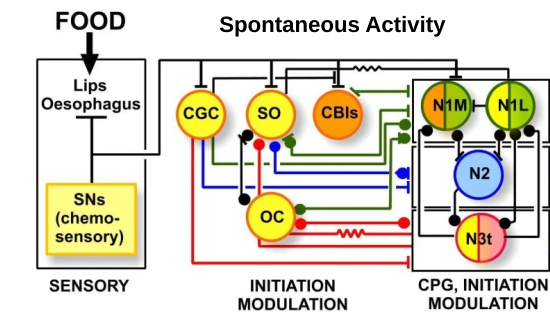
\includegraphics[width=0.5\textwidth]{img/invariants/data/SUSSEX/Summary/distributed_benjamin_2012_spon.png} % The overlapping image
		}
		\end{overpic}
	\end{minipage}
	\begin{minipage}{0.49\textwidth}
		\centering
		\begin{overpic}[width=\textwidth]{img/invariants/data/SUSSEX/Summary/output_pairplot_so.pdf} % Base image
			\put(50,55){ % Position the second image (70%, 60% of width/height of figure1)
				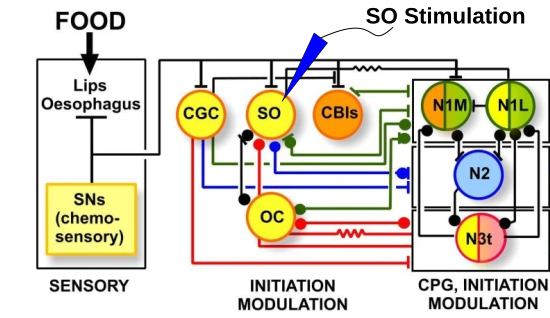
\includegraphics[width=0.5\textwidth]{img/invariants/data/SUSSEX/Summary/distributed_benjamin_2012_so.png} % The overlapping image
			}
		\end{overpic}
	\end{minipage}
\end{minipage}

\begin{minipage}{\textwidth}
	\begin{minipage}{0.49\textwidth}
		\centering
		\begin{overpic}[width=\textwidth]{img/invariants/data/SUSSEX/Summary/output_pairplot_mln.pdf} % Base image
			\put(50,55){ % Position the second image (70%, 60% of width/height of figure1)
				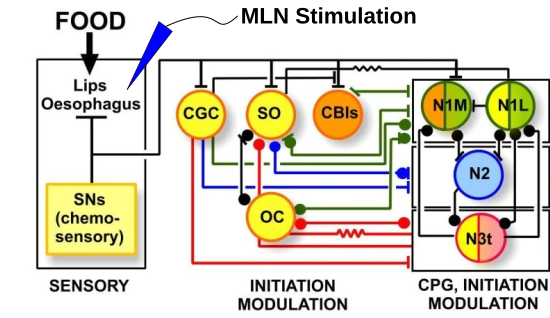
\includegraphics[width=0.5\textwidth]{img/invariants/data/SUSSEX/Summary/distributed_benjamin_2012_mln.png} % The overlapping image
			}
		\end{overpic}
	\end{minipage}	
	\begin{minipage}{0.49\textwidth}
		\centering
		\begin{overpic}[width=\textwidth]{img/invariants/data/SUSSEX/Summary/output_pairplot_cv1a.pdf} % Base image
			\put(50,55){ % Position the second image (70%, 60% of width/height of figure1)
				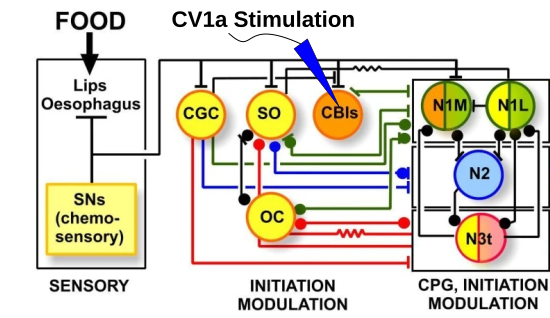
\includegraphics[width=0.5\textwidth]{img/invariants/data/SUSSEX/Summary/distributed_benjamin_2012_cv1a.png} % The overlapping image
			}
		\end{overpic}
	\end{minipage}
\end{minipage}

\caption{Summary of the results discussed for different rhythm modulations. Each pairplot shows all possible interval combinations, the upper right connection diagram shows the neuron stimulated for each case. The examples shown here correspond to (from left to right and top to bottom): Spontaneous activity example 1 (Fig. \ref{fig:prep2 invariants}), SO induced modulation (Fig. \ref{fig:so induced invariants}), MLN stimulation (Fig. \ref{fig:mln stimulation}) and CVa1 stimulation (Fig. \ref{fig:cv1a 1 2phases}).}
\label{fig:results summary}
	
\end{figure}

\clearpage

\subsection{Invariant resetting}
There is another important feature of the sequential dynamical invariants reported in \textcite{elices_robust_2019}: there is no relation between time intervals belonging to different cycles. In the model, the study of these phenomena was not possible since the current ramp provided a gradual change of the time-intervals' duration, which forced all intervals correlated in a cycle to be also correlated in the next one (see Appendix Fig. \ref{fig:N1M stimulation pairplot reset}). 

In this subsection, we include several experimental examples of this invariant resetting for cases presenting robust sequential dynamical invariants. We illustrate this "reset" with pairplots gathering the interval relations of a given cycle in the bottom triangle sector (below the diagonal indicated by a dashed line), and the relations of each interval with those of the next cycle represented in the upper triangle (Fig. \ref{fig:reset pairplot comparison}). When comparing intervals of one cycle to those of the next one, existing robust  correlations disappear, the most clear example is illustrated in the first figure for the spontaneous activity. All strong linear interval relationships are gone when intervals between consecutive cycles are compared, with $R^2$ close to 0. In the two examples illustrated in the second row, i.e., MLN stimulation and CV1a stimulation recordings, what were strong linear relations are diluted and a few new strong correlations appear between intervals of consecutive cycles, but note that none of them existed between those intervals in the same cycle. For example, the robust dynamical invariant between N1 burst duration and the period is diluted when comparing the relation for consecutive cycles in both cases. Strong correlations are present between N1 and N3 periods and between N1 burst duration and N3 period. Both periods overlap between cycles, which can explain the relation that appears between intervals of consecutive cycles. Therefore, robust dynamical invariants in the form of related interval variability exist only between specific intervals of the same cycle, and they are not propagated between cycles. Time intervals that overlap between consecutive cycles can be related.


\begin{figure}[htbp]
	\centering
	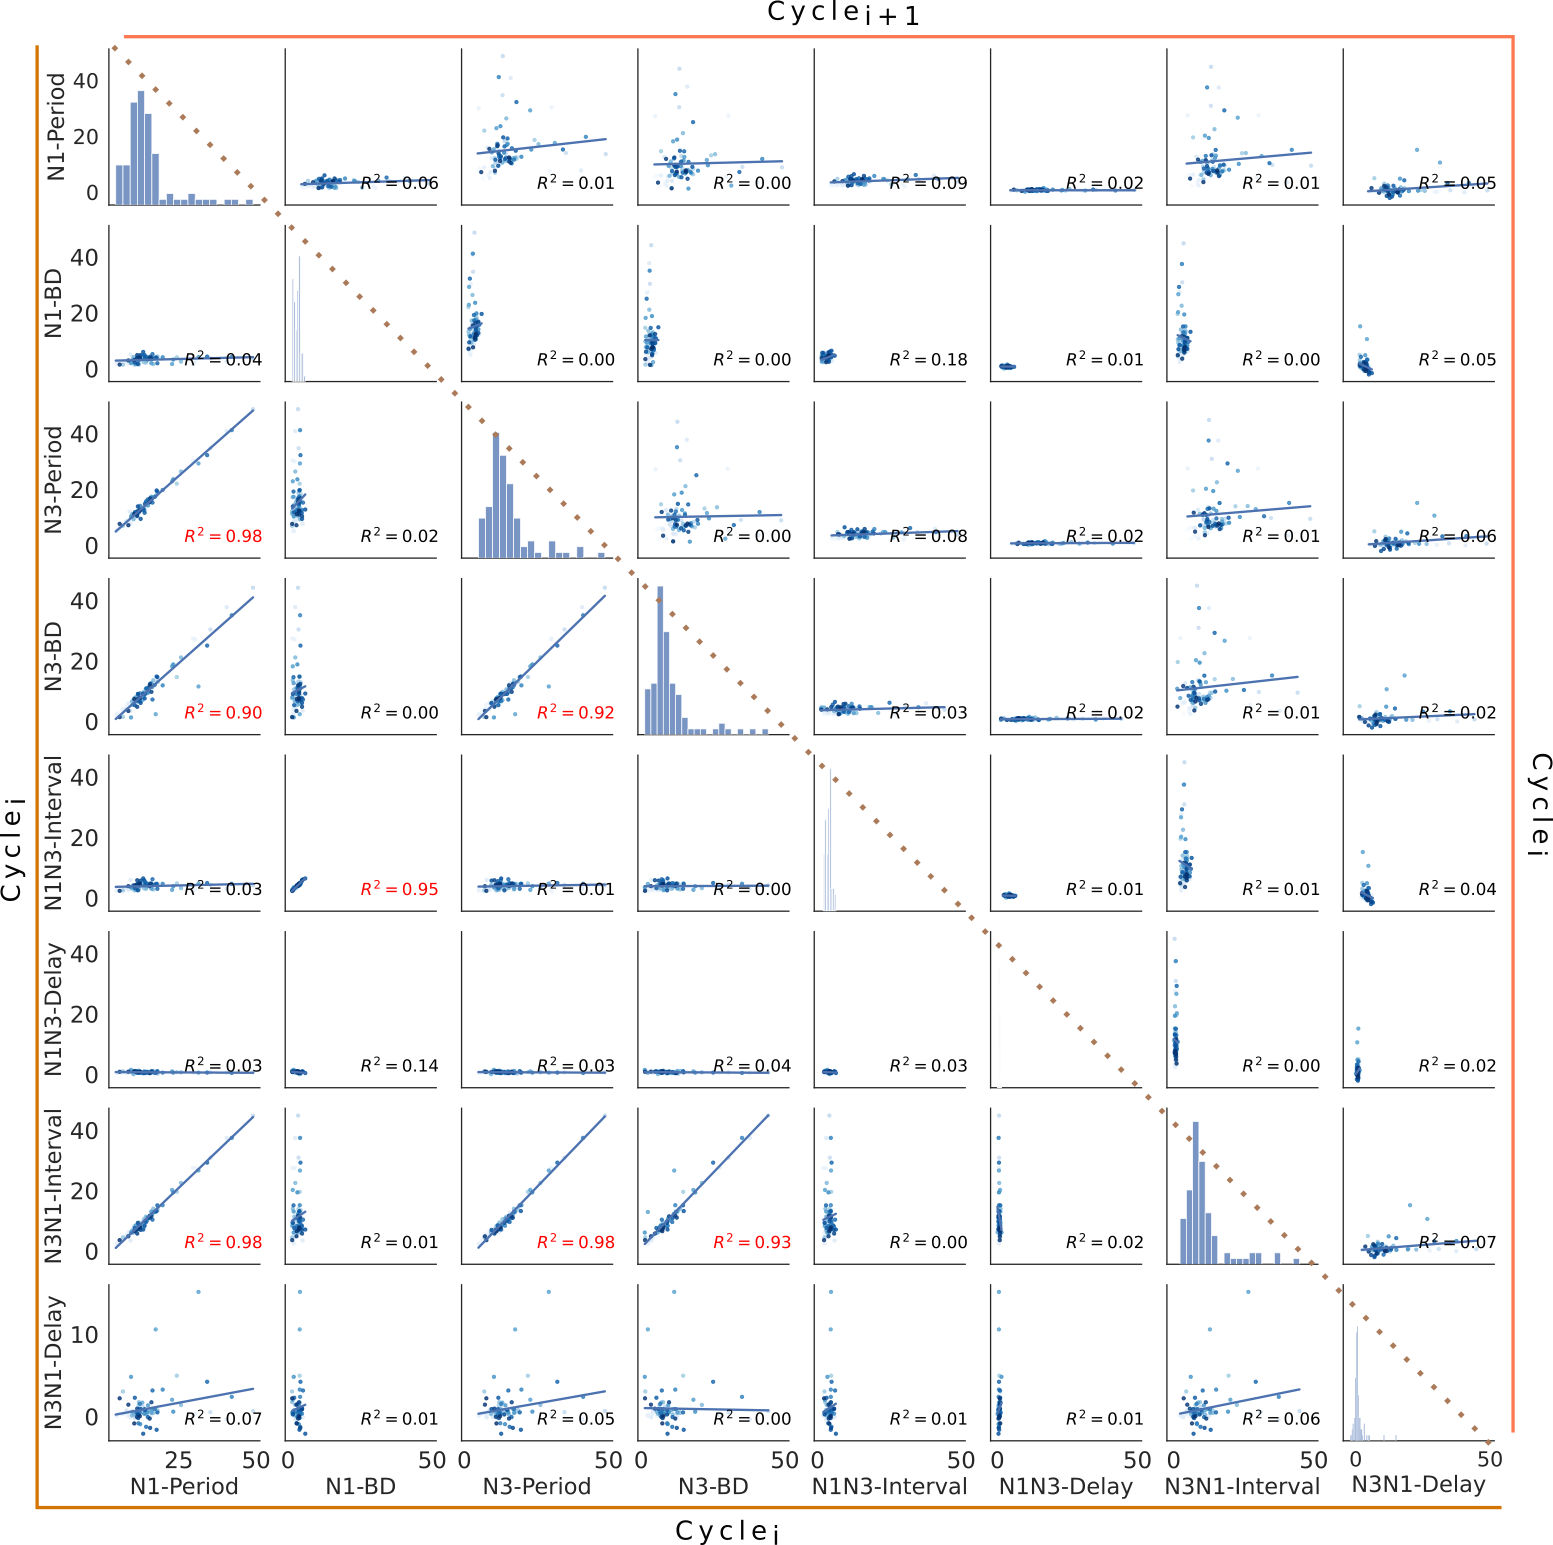
\includegraphics[width=0.49\textwidth]{./img/invariants/data/SUSSEX/prep2/images/2phases/output_pairplot_reset_triangle.png}
	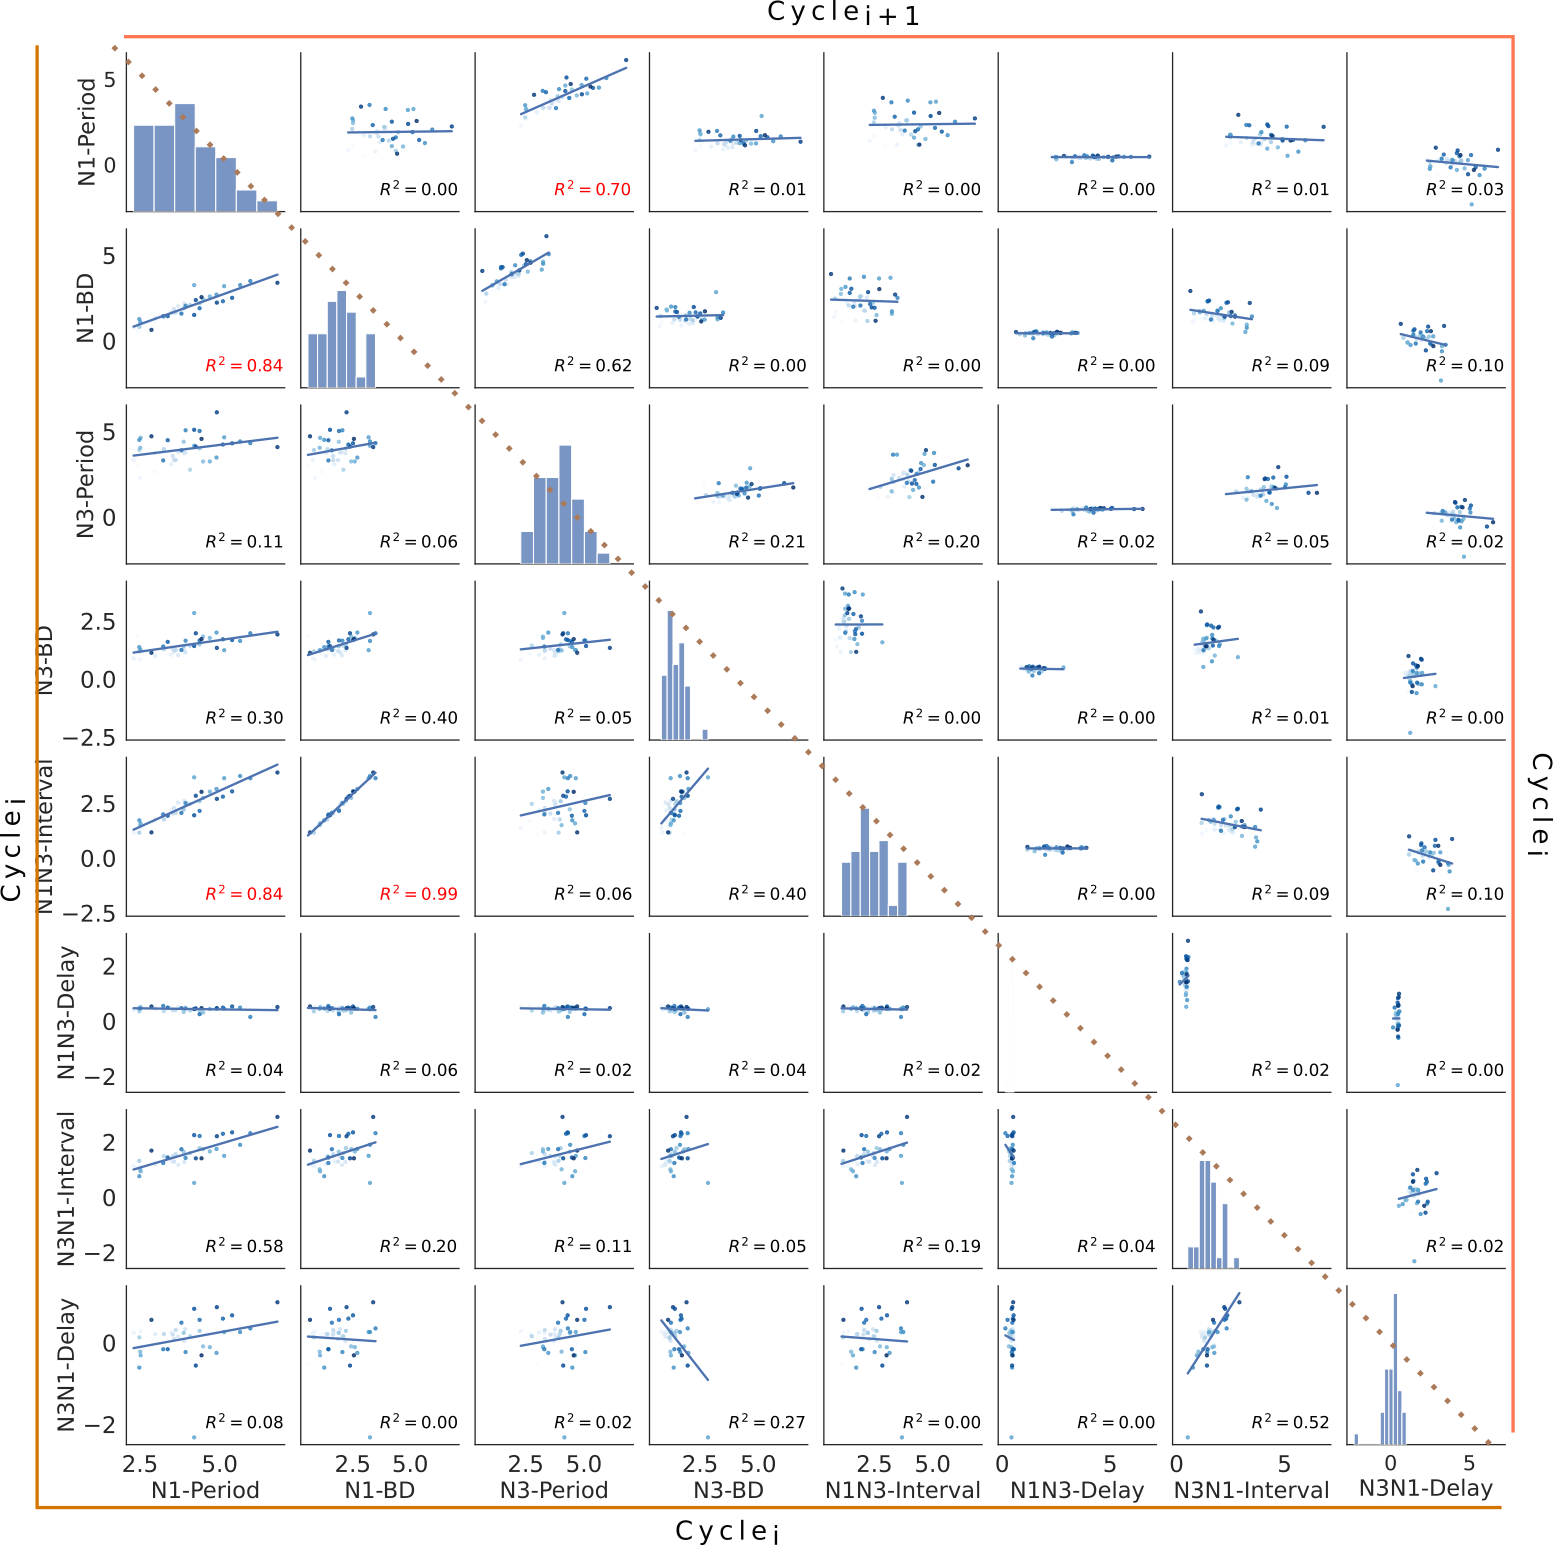
\includegraphics[width=0.49\textwidth]{./img/invariants/data/SUSSEX/SO_driven/images/output_pairplot_reset_triangle.png}
    \\
    \vspace{10pt}
	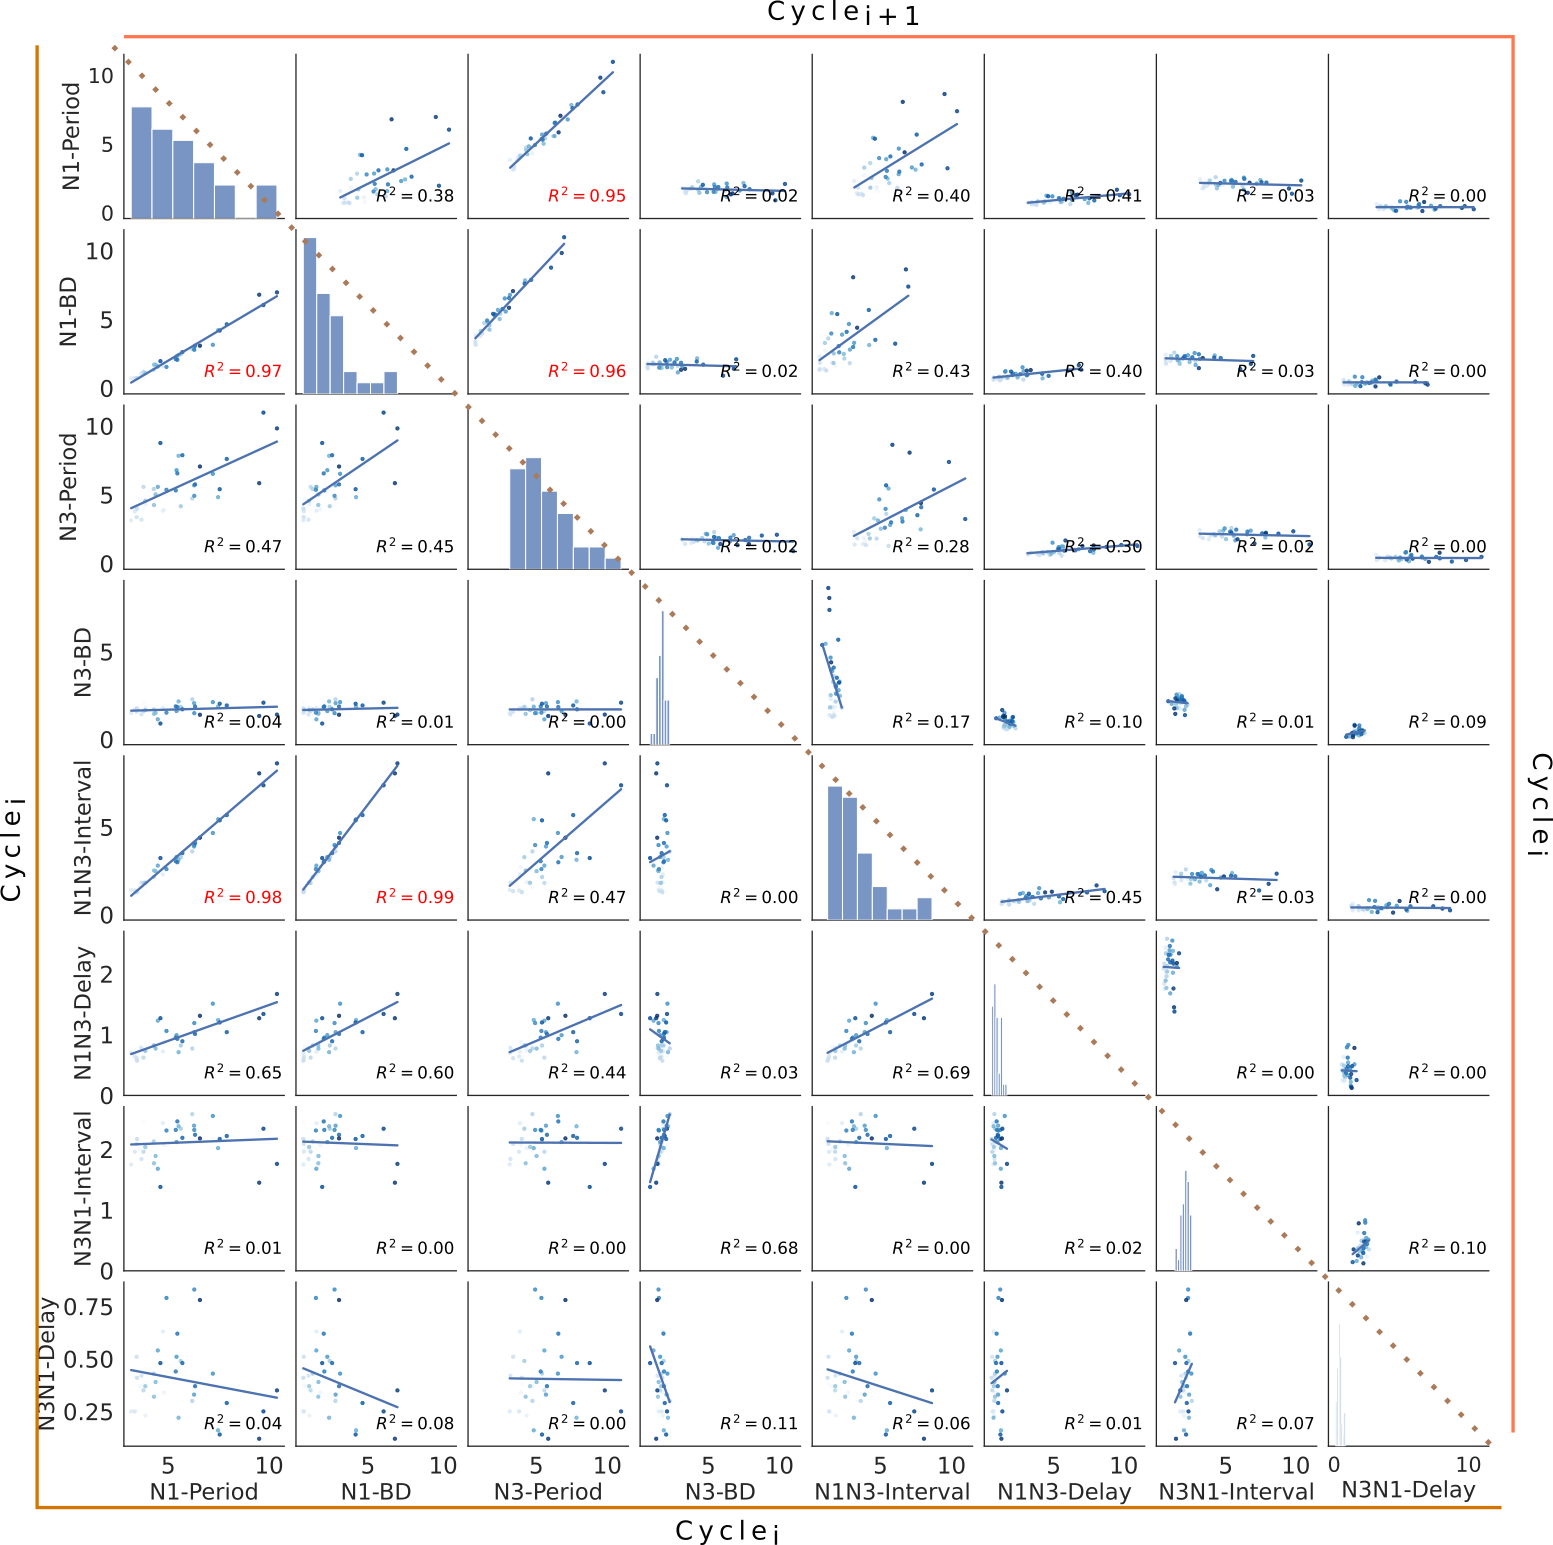
\includegraphics[width=0.49\textwidth]{./img/invariants/data/SUSSEX/MLN_driven/images/output_pairplot_reset_triangle.png}
	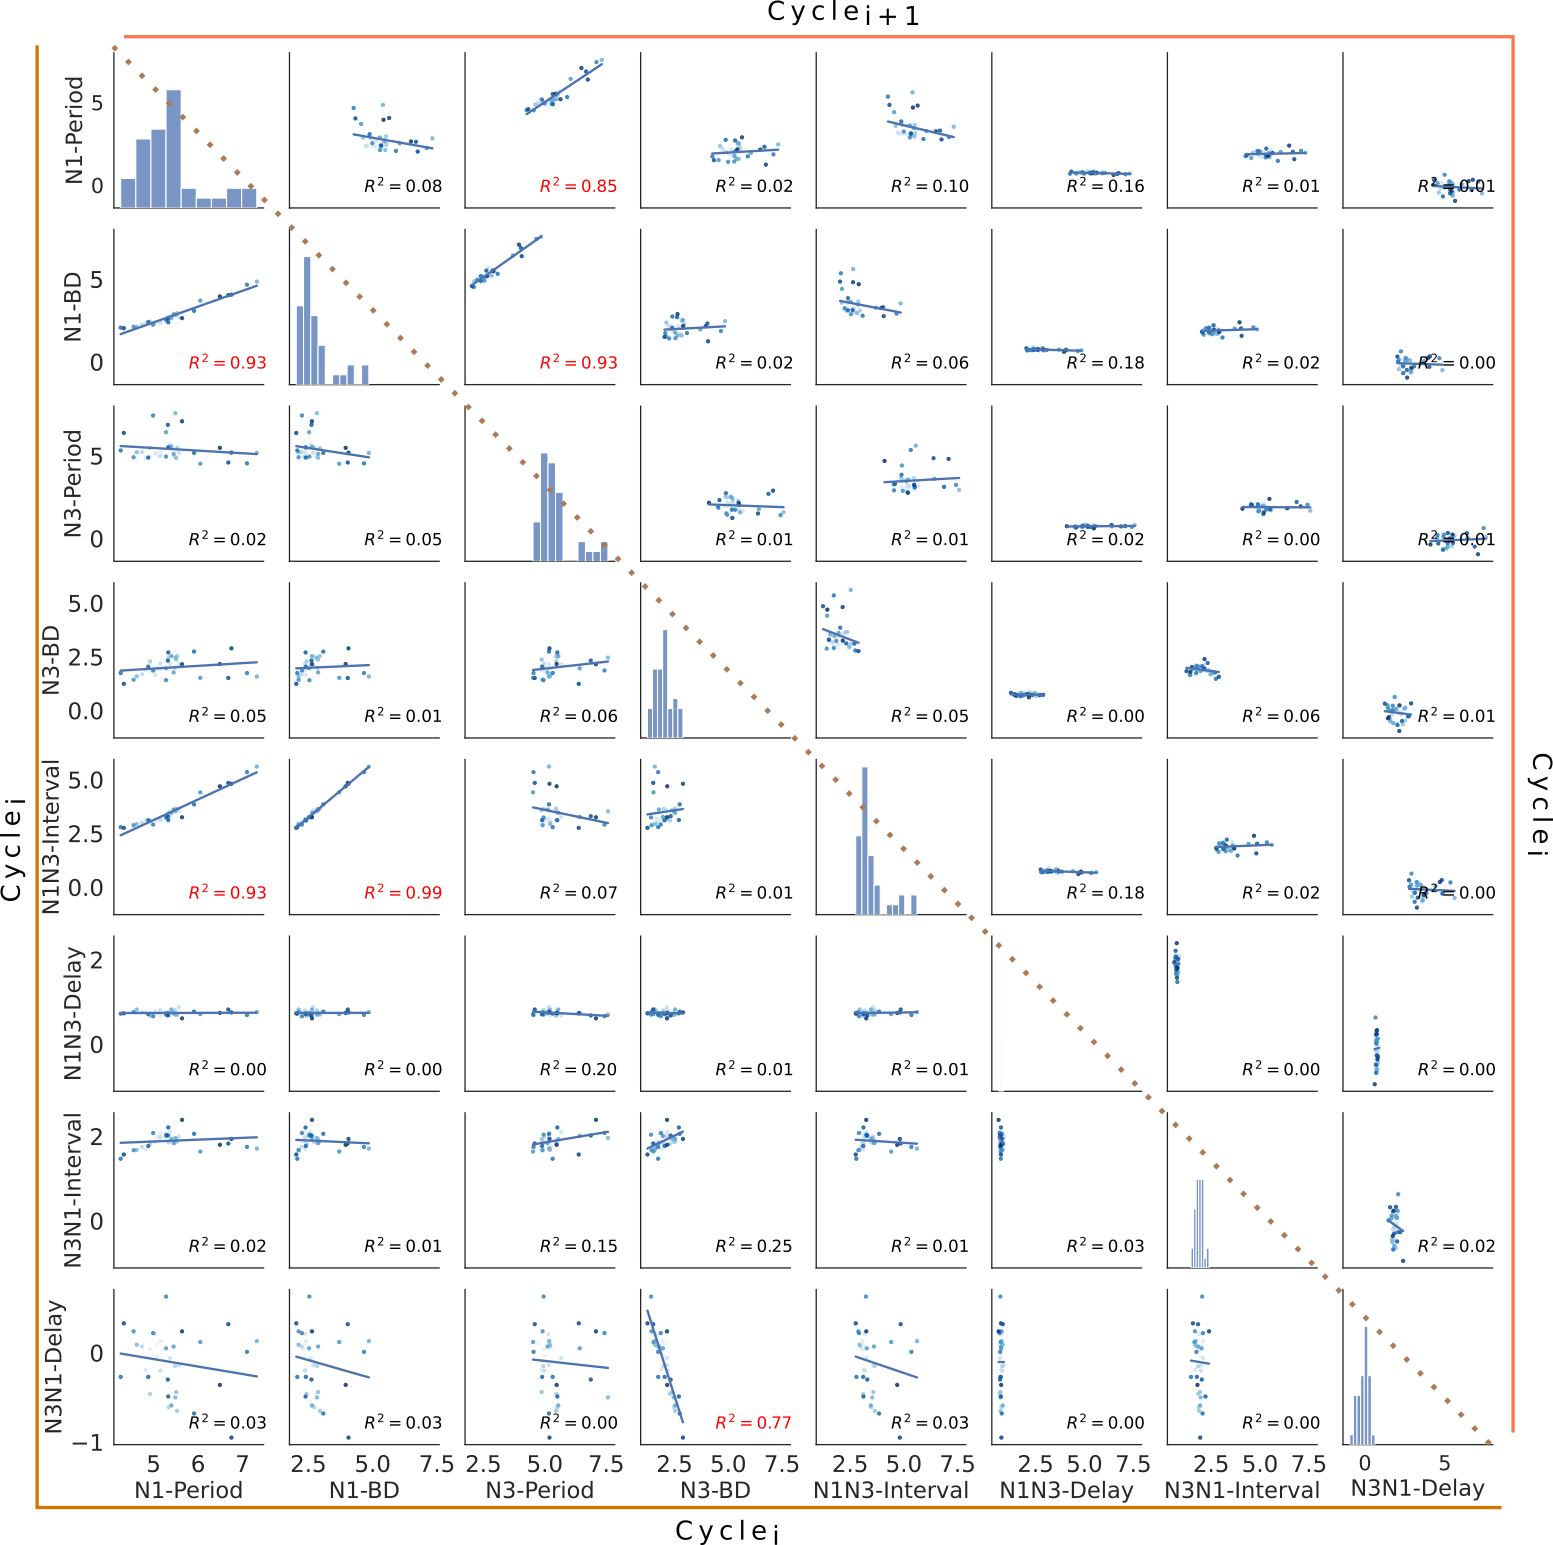
\includegraphics[width=0.49\textwidth]{./img/invariants/data/SUSSEX/CV1a_driven1/images/2phases/output_pairplot_reset_triangle.png}
	\caption{Absence of dynamical invariants between non-overlapping intervals in consecutive cycles. For each pairplot, the lower triangle represents interval relationships in the same cycle and the upper triangle represents relationships between intervals of one cycle against  intervals of the next cycle. The examples shown here correspond to (from left to right and top to bottom): Spontaneous activity example 1 (Fig. \ref{fig:prep2 invariants}), SO induced modulation (Fig. \ref{fig:so induced invariants}), MLN stimulation (Fig. \ref{fig:mln stimulation}) and CVa1 stimulation (Fig. \ref{fig:cv1a 1 2phases}).}
	\label{fig:reset pairplot comparison}
\end{figure}

\clearpage
\newpage
